% Options for packages loaded elsewhere
\PassOptionsToPackage{unicode}{hyperref}
\PassOptionsToPackage{hyphens}{url}
\PassOptionsToPackage{dvipsnames,svgnames,x11names}{xcolor}
%
\documentclass[
  letterpaper,
  DIV=11,
  numbers=noendperiod]{scrreprt}

\usepackage{amsmath,amssymb}
\usepackage{iftex}
\ifPDFTeX
  \usepackage[T1]{fontenc}
  \usepackage[utf8]{inputenc}
  \usepackage{textcomp} % provide euro and other symbols
\else % if luatex or xetex
  \usepackage{unicode-math}
  \defaultfontfeatures{Scale=MatchLowercase}
  \defaultfontfeatures[\rmfamily]{Ligatures=TeX,Scale=1}
\fi
\usepackage{lmodern}
\ifPDFTeX\else  
    % xetex/luatex font selection
\fi
% Use upquote if available, for straight quotes in verbatim environments
\IfFileExists{upquote.sty}{\usepackage{upquote}}{}
\IfFileExists{microtype.sty}{% use microtype if available
  \usepackage[]{microtype}
  \UseMicrotypeSet[protrusion]{basicmath} % disable protrusion for tt fonts
}{}
\makeatletter
\@ifundefined{KOMAClassName}{% if non-KOMA class
  \IfFileExists{parskip.sty}{%
    \usepackage{parskip}
  }{% else
    \setlength{\parindent}{0pt}
    \setlength{\parskip}{6pt plus 2pt minus 1pt}}
}{% if KOMA class
  \KOMAoptions{parskip=half}}
\makeatother
\usepackage{xcolor}
\setlength{\emergencystretch}{3em} % prevent overfull lines
\setcounter{secnumdepth}{5}
% Make \paragraph and \subparagraph free-standing
\ifx\paragraph\undefined\else
  \let\oldparagraph\paragraph
  \renewcommand{\paragraph}[1]{\oldparagraph{#1}\mbox{}}
\fi
\ifx\subparagraph\undefined\else
  \let\oldsubparagraph\subparagraph
  \renewcommand{\subparagraph}[1]{\oldsubparagraph{#1}\mbox{}}
\fi

\usepackage{color}
\usepackage{fancyvrb}
\newcommand{\VerbBar}{|}
\newcommand{\VERB}{\Verb[commandchars=\\\{\}]}
\DefineVerbatimEnvironment{Highlighting}{Verbatim}{commandchars=\\\{\}}
% Add ',fontsize=\small' for more characters per line
\usepackage{framed}
\definecolor{shadecolor}{RGB}{241,243,245}
\newenvironment{Shaded}{\begin{snugshade}}{\end{snugshade}}
\newcommand{\AlertTok}[1]{\textcolor[rgb]{0.68,0.00,0.00}{#1}}
\newcommand{\AnnotationTok}[1]{\textcolor[rgb]{0.37,0.37,0.37}{#1}}
\newcommand{\AttributeTok}[1]{\textcolor[rgb]{0.40,0.45,0.13}{#1}}
\newcommand{\BaseNTok}[1]{\textcolor[rgb]{0.68,0.00,0.00}{#1}}
\newcommand{\BuiltInTok}[1]{\textcolor[rgb]{0.00,0.23,0.31}{#1}}
\newcommand{\CharTok}[1]{\textcolor[rgb]{0.13,0.47,0.30}{#1}}
\newcommand{\CommentTok}[1]{\textcolor[rgb]{0.37,0.37,0.37}{#1}}
\newcommand{\CommentVarTok}[1]{\textcolor[rgb]{0.37,0.37,0.37}{\textit{#1}}}
\newcommand{\ConstantTok}[1]{\textcolor[rgb]{0.56,0.35,0.01}{#1}}
\newcommand{\ControlFlowTok}[1]{\textcolor[rgb]{0.00,0.23,0.31}{#1}}
\newcommand{\DataTypeTok}[1]{\textcolor[rgb]{0.68,0.00,0.00}{#1}}
\newcommand{\DecValTok}[1]{\textcolor[rgb]{0.68,0.00,0.00}{#1}}
\newcommand{\DocumentationTok}[1]{\textcolor[rgb]{0.37,0.37,0.37}{\textit{#1}}}
\newcommand{\ErrorTok}[1]{\textcolor[rgb]{0.68,0.00,0.00}{#1}}
\newcommand{\ExtensionTok}[1]{\textcolor[rgb]{0.00,0.23,0.31}{#1}}
\newcommand{\FloatTok}[1]{\textcolor[rgb]{0.68,0.00,0.00}{#1}}
\newcommand{\FunctionTok}[1]{\textcolor[rgb]{0.28,0.35,0.67}{#1}}
\newcommand{\ImportTok}[1]{\textcolor[rgb]{0.00,0.46,0.62}{#1}}
\newcommand{\InformationTok}[1]{\textcolor[rgb]{0.37,0.37,0.37}{#1}}
\newcommand{\KeywordTok}[1]{\textcolor[rgb]{0.00,0.23,0.31}{#1}}
\newcommand{\NormalTok}[1]{\textcolor[rgb]{0.00,0.23,0.31}{#1}}
\newcommand{\OperatorTok}[1]{\textcolor[rgb]{0.37,0.37,0.37}{#1}}
\newcommand{\OtherTok}[1]{\textcolor[rgb]{0.00,0.23,0.31}{#1}}
\newcommand{\PreprocessorTok}[1]{\textcolor[rgb]{0.68,0.00,0.00}{#1}}
\newcommand{\RegionMarkerTok}[1]{\textcolor[rgb]{0.00,0.23,0.31}{#1}}
\newcommand{\SpecialCharTok}[1]{\textcolor[rgb]{0.37,0.37,0.37}{#1}}
\newcommand{\SpecialStringTok}[1]{\textcolor[rgb]{0.13,0.47,0.30}{#1}}
\newcommand{\StringTok}[1]{\textcolor[rgb]{0.13,0.47,0.30}{#1}}
\newcommand{\VariableTok}[1]{\textcolor[rgb]{0.07,0.07,0.07}{#1}}
\newcommand{\VerbatimStringTok}[1]{\textcolor[rgb]{0.13,0.47,0.30}{#1}}
\newcommand{\WarningTok}[1]{\textcolor[rgb]{0.37,0.37,0.37}{\textit{#1}}}

\providecommand{\tightlist}{%
  \setlength{\itemsep}{0pt}\setlength{\parskip}{0pt}}\usepackage{longtable,booktabs,array}
\usepackage{calc} % for calculating minipage widths
% Correct order of tables after \paragraph or \subparagraph
\usepackage{etoolbox}
\makeatletter
\patchcmd\longtable{\par}{\if@noskipsec\mbox{}\fi\par}{}{}
\makeatother
% Allow footnotes in longtable head/foot
\IfFileExists{footnotehyper.sty}{\usepackage{footnotehyper}}{\usepackage{footnote}}
\makesavenoteenv{longtable}
\usepackage{graphicx}
\makeatletter
\def\maxwidth{\ifdim\Gin@nat@width>\linewidth\linewidth\else\Gin@nat@width\fi}
\def\maxheight{\ifdim\Gin@nat@height>\textheight\textheight\else\Gin@nat@height\fi}
\makeatother
% Scale images if necessary, so that they will not overflow the page
% margins by default, and it is still possible to overwrite the defaults
% using explicit options in \includegraphics[width, height, ...]{}
\setkeys{Gin}{width=\maxwidth,height=\maxheight,keepaspectratio}
% Set default figure placement to htbp
\makeatletter
\def\fps@figure{htbp}
\makeatother
\newlength{\cslhangindent}
\setlength{\cslhangindent}{1.5em}
\newlength{\csllabelwidth}
\setlength{\csllabelwidth}{3em}
\newlength{\cslentryspacingunit} % times entry-spacing
\setlength{\cslentryspacingunit}{\parskip}
\newenvironment{CSLReferences}[2] % #1 hanging-ident, #2 entry spacing
 {% don't indent paragraphs
  \setlength{\parindent}{0pt}
  % turn on hanging indent if param 1 is 1
  \ifodd #1
  \let\oldpar\par
  \def\par{\hangindent=\cslhangindent\oldpar}
  \fi
  % set entry spacing
  \setlength{\parskip}{#2\cslentryspacingunit}
 }%
 {}
\usepackage{calc}
\newcommand{\CSLBlock}[1]{#1\hfill\break}
\newcommand{\CSLLeftMargin}[1]{\parbox[t]{\csllabelwidth}{#1}}
\newcommand{\CSLRightInline}[1]{\parbox[t]{\linewidth - \csllabelwidth}{#1}\break}
\newcommand{\CSLIndent}[1]{\hspace{\cslhangindent}#1}

\KOMAoption{captions}{tableheading}
\makeatletter
\makeatother
\makeatletter
\@ifpackageloaded{bookmark}{}{\usepackage{bookmark}}
\makeatother
\makeatletter
\@ifpackageloaded{caption}{}{\usepackage{caption}}
\AtBeginDocument{%
\ifdefined\contentsname
  \renewcommand*\contentsname{Table of contents}
\else
  \newcommand\contentsname{Table of contents}
\fi
\ifdefined\listfigurename
  \renewcommand*\listfigurename{List of Figures}
\else
  \newcommand\listfigurename{List of Figures}
\fi
\ifdefined\listtablename
  \renewcommand*\listtablename{List of Tables}
\else
  \newcommand\listtablename{List of Tables}
\fi
\ifdefined\figurename
  \renewcommand*\figurename{Figure}
\else
  \newcommand\figurename{Figure}
\fi
\ifdefined\tablename
  \renewcommand*\tablename{Table}
\else
  \newcommand\tablename{Table}
\fi
}
\@ifpackageloaded{float}{}{\usepackage{float}}
\floatstyle{ruled}
\@ifundefined{c@chapter}{\newfloat{codelisting}{h}{lop}}{\newfloat{codelisting}{h}{lop}[chapter]}
\floatname{codelisting}{Listing}
\newcommand*\listoflistings{\listof{codelisting}{List of Listings}}
\makeatother
\makeatletter
\@ifpackageloaded{caption}{}{\usepackage{caption}}
\@ifpackageloaded{subcaption}{}{\usepackage{subcaption}}
\makeatother
\makeatletter
\@ifpackageloaded{tcolorbox}{}{\usepackage[skins,breakable]{tcolorbox}}
\makeatother
\makeatletter
\@ifundefined{shadecolor}{\definecolor{shadecolor}{rgb}{.97, .97, .97}}
\makeatother
\makeatletter
\makeatother
\makeatletter
\makeatother
\ifLuaTeX
  \usepackage{selnolig}  % disable illegal ligatures
\fi
\IfFileExists{bookmark.sty}{\usepackage{bookmark}}{\usepackage{hyperref}}
\IfFileExists{xurl.sty}{\usepackage{xurl}}{} % add URL line breaks if available
\urlstyle{same} % disable monospaced font for URLs
\hypersetup{
  pdftitle={Statistical Methods for Composite Endpoints},
  pdfauthor={Lu Mao},
  colorlinks=true,
  linkcolor={blue},
  filecolor={Maroon},
  citecolor={Blue},
  urlcolor={Blue},
  pdfcreator={LaTeX via pandoc}}

\title{Statistical Methods for Composite Endpoints}
\usepackage{etoolbox}
\makeatletter
\providecommand{\subtitle}[1]{% add subtitle to \maketitle
  \apptocmd{\@title}{\par {\large #1 \par}}{}{}
}
\makeatother
\subtitle{Win Ratio and Beyond}
\author{Lu Mao}
\date{}

\begin{document}
\maketitle
\ifdefined\Shaded\renewenvironment{Shaded}{\begin{tcolorbox}[interior hidden, enhanced, sharp corners, boxrule=0pt, frame hidden, breakable, borderline west={3pt}{0pt}{shadecolor}]}{\end{tcolorbox}}\fi

\renewcommand*\contentsname{Table of contents}
{
\hypersetup{linkcolor=}
\setcounter{tocdepth}{2}
\tableofcontents
}
\bookmarksetup{startatroot}

\hypertarget{course-info}{%
\chapter*{Course Info}\label{course-info}}
\addcontentsline{toc}{chapter}{Course Info}

\markboth{Course Info}{Course Info}

This is a companion site for the same-titled \textbf{workshop} at the
\href{https://www.sctweb.org/meeting/}{2024 Society for Clinical Trials
(SCT) Annual Meeting} given on May 19, 2024 at Boston Marriott Copley
Place
(\href{https://www.google.com/maps/place/Boston+Marriott+Copley+Place/@42.3467509,-71.0815269,17z/data=!3m1!5s0x89e37a0d93723ac1:0x7edf0a3a678073b5!4m10!3m9!1s0x89e37a0de7e77a4b:0x1a77f7939c6472fb!5m3!1s2024-07-28!4m1!1i2!8m2!3d42.346747!4d-71.078952!16s\%2Fm\%2F0wfgs85?entry=ttu}{map})
in Boston, MA.

\hypertarget{time-and-place}{%
\section*{Time and Place}\label{time-and-place}}
\addcontentsline{toc}{section}{Time and Place}

\markright{Time and Place}

\begin{itemize}
\tightlist
\item
  Sun, May 19 \textbar{} 8:00 AM - 12:00 PM
\item
  Room: Suffolk (3rd Floor)
\end{itemize}

\hypertarget{instructor-profile}{%
\section*{Instructor Profile}\label{instructor-profile}}
\addcontentsline{toc}{section}{Instructor Profile}

\markright{Instructor Profile}

\href{https://sites.google.com/view/lmaowisc}{Lu Mao, PhD}

\begin{itemize}
\tightlist
\item
  Associate Professor of Biostatistics at UW-Madison
\item
  Methodologic research

  \begin{itemize}
  \tightlist
  \item
    \href{https://reporter.nih.gov/search/9aSu5u3xlE26GrjbF_4cBg/project-details/10734551}{R01HL149875}:
    \emph{Novel Statistical Methods for Complex Time-to-Event Data in
    Cardiovascular Clinical Trials} (12/01/2019 -- 07/31/2028)
  \item
    \href{https://www.nsf.gov/awardsearch/showAward?AWD_ID=2015526}{DMS2015526}:
    \emph{Randomized Trials with Non-Compliance} (07/01/2020 --
    06/30/2024)
  \end{itemize}
\item
  Collaborative research

  \begin{itemize}
  \tightlist
  \item
    Cardiovascular disease, cancer, radiology, behavioral health
    interventions
  \end{itemize}
\item
  Teaching

  \begin{itemize}
  \tightlist
  \item
    \href{https://lmaowisc.github.io/BMI741}{Survival Analysis: Theory
    and Methods} (UW; 2020 - 2024)
  \end{itemize}
\item
  Editorial service

  \begin{itemize}
  \tightlist
  \item
    \href{https://www.jacc.org/journal/heart-failure/editorial-board}{Statistical
    Editor}, \emph{JACC Journals}
  \item
    \href{https://www.tandfonline.com/action/journalInformation?show=editorialBoard\&journalCode=usbr20}{Associate
    Editor}, \emph{Statistics for Biopharmaceutical Research}
  \end{itemize}
\end{itemize}

\hypertarget{learning-outcomes}{%
\section*{Learning Outcomes}\label{learning-outcomes}}
\addcontentsline{toc}{section}{Learning Outcomes}

\markright{Learning Outcomes}

\begin{itemize}
\tightlist
\item
  Understand the statistical and scientific challenges with composite
  endpoints as well as regulatory guidelines/requirements
\item
  Learn the basics of statistical methodology, e.g., testing, power
  analysis, nonparametric estimation, and semiparametric regression to
  address these challenges
\item
  Get hands-on experience with real data using publicly available
  R-packages
\end{itemize}

\hypertarget{syllabus}{%
\section*{Syllabus}\label{syllabus}}
\addcontentsline{toc}{section}{Syllabus}

\markright{Syllabus}

\begin{itemize}
\tightlist
\item
  \textbf{1. Introduction} (30 min)

  \begin{itemize}
  \tightlist
  \item
    1.1 Examples \& guidelines
  \item
    1.2 Traditional methods and limitations
  \item
    1.3 Win ratio methods and limitations
  \end{itemize}
\item
  \textbf{2. Hypothesis Testing} (40 min)

  \begin{itemize}
  \tightlist
  \item
    2.1 Win ratio by Pocock et al.~(2012)
  \item
    2.2 Statistical properties
  \item
    2.3 Handling recurrent events (R-package
    \href{https://cran.r-project.org/package=WR}{\texttt{WR}})
  \item
    2.4 Sample size calculation (R-package
    \href{https://cran.r-project.org/package=WR}{\texttt{WR}})
  \end{itemize}
\item
  \textbf{3. Nonparametric Estimation} (60 min)

  \begin{itemize}
  \tightlist
  \item
    3.1 Restricted win ratio
  \item
    3.2 Average win time analysis (R-package
    \href{https://cran.r-project.org/package=rmt}{\texttt{rmt}})

    \begin{itemize}
    \tightlist
    \item
      3.1.1 Restricted mean time in favor of treatment
    \item
      3.1.2 Estimation, inference, and graphics
    \item
      3.1.3 Real Examples
    \end{itemize}
  \item
    3.3 While-alive loss rate (R-package
    \href{https://cran.r-project.org/package=WA}{\texttt{WA}})

    \begin{itemize}
    \tightlist
    \item
      3.2.1 Definition, interpretation, and estimation
    \item
      3.2.3 Real Examples
    \end{itemize}
  \end{itemize}
\item
  \textbf{4. Semiparametric Regression} (30 min)

  \begin{itemize}
  \tightlist
  \item
    4.1 Proportional win-fractions model (R-package
    \href{https://cran.r-project.org/package=WR}{\texttt{WR}})

    \begin{itemize}
    \tightlist
    \item
      4.1.1 Model assumptions
    \item
      4.1.2 Estimation, inference, and model diagnostics
    \item
      4.1.3 Real Examples
    \end{itemize}
  \item
    4.2 Generalized proportional odds model (tentative)

    \begin{itemize}
    \tightlist
    \item
      4.2.1 Model specification and possible estimation
    \end{itemize}
  \end{itemize}
\item
  \textbf{5. Discussions} (20 min)

  \begin{itemize}
  \tightlist
  \item
    5.1. Course summary
  \item
    5.2. Future work

    \begin{itemize}
    \tightlist
    \item
      5.2.1 Covariate adjustment
    \item
      5.2.2 Intercurrent events
    \end{itemize}
  \end{itemize}
\end{itemize}

\hypertarget{r-packages}{%
\section*{R-Packages}\label{r-packages}}
\addcontentsline{toc}{section}{R-Packages}

\markright{R-Packages}

To proceed, install/load the following packages:

\begin{Shaded}
\begin{Highlighting}[]
\CommentTok{\# install packages {-}{-}{-}{-}{-}{-}{-}{-}{-}{-}{-}{-}{-}{-}{-}{-}{-}{-}{-}{-}{-}{-}{-}{-}{-}{-}{-}{-}{-}{-}{-}{-}}
\FunctionTok{install.packages}\NormalTok{(}\StringTok{"Wcompo"}\NormalTok{)}
\FunctionTok{install.packages}\NormalTok{(}\StringTok{"WR"}\NormalTok{)}
\FunctionTok{install.packages}\NormalTok{(}\StringTok{"rmt"}\NormalTok{)}
\FunctionTok{install.packages}\NormalTok{(}\StringTok{"WA"}\NormalTok{)}
\CommentTok{\# load packages {-}{-}{-}{-}{-}{-}{-}{-}{-}{-}{-}{-}{-}{-}{-}{-}{-}{-}{-}{-}{-}{-}{-}{-}{-}{-}{-}{-}{-}{-}{-}{-}{-}{-}{-}}
\FunctionTok{library}\NormalTok{(tidyverse)}
\FunctionTok{library}\NormalTok{(survival)}
\FunctionTok{library}\NormalTok{(Wcompo)}
\FunctionTok{library}\NormalTok{(WR)}
\FunctionTok{library}\NormalTok{(rmt)}
\FunctionTok{library}\NormalTok{(WA)}
\end{Highlighting}
\end{Shaded}

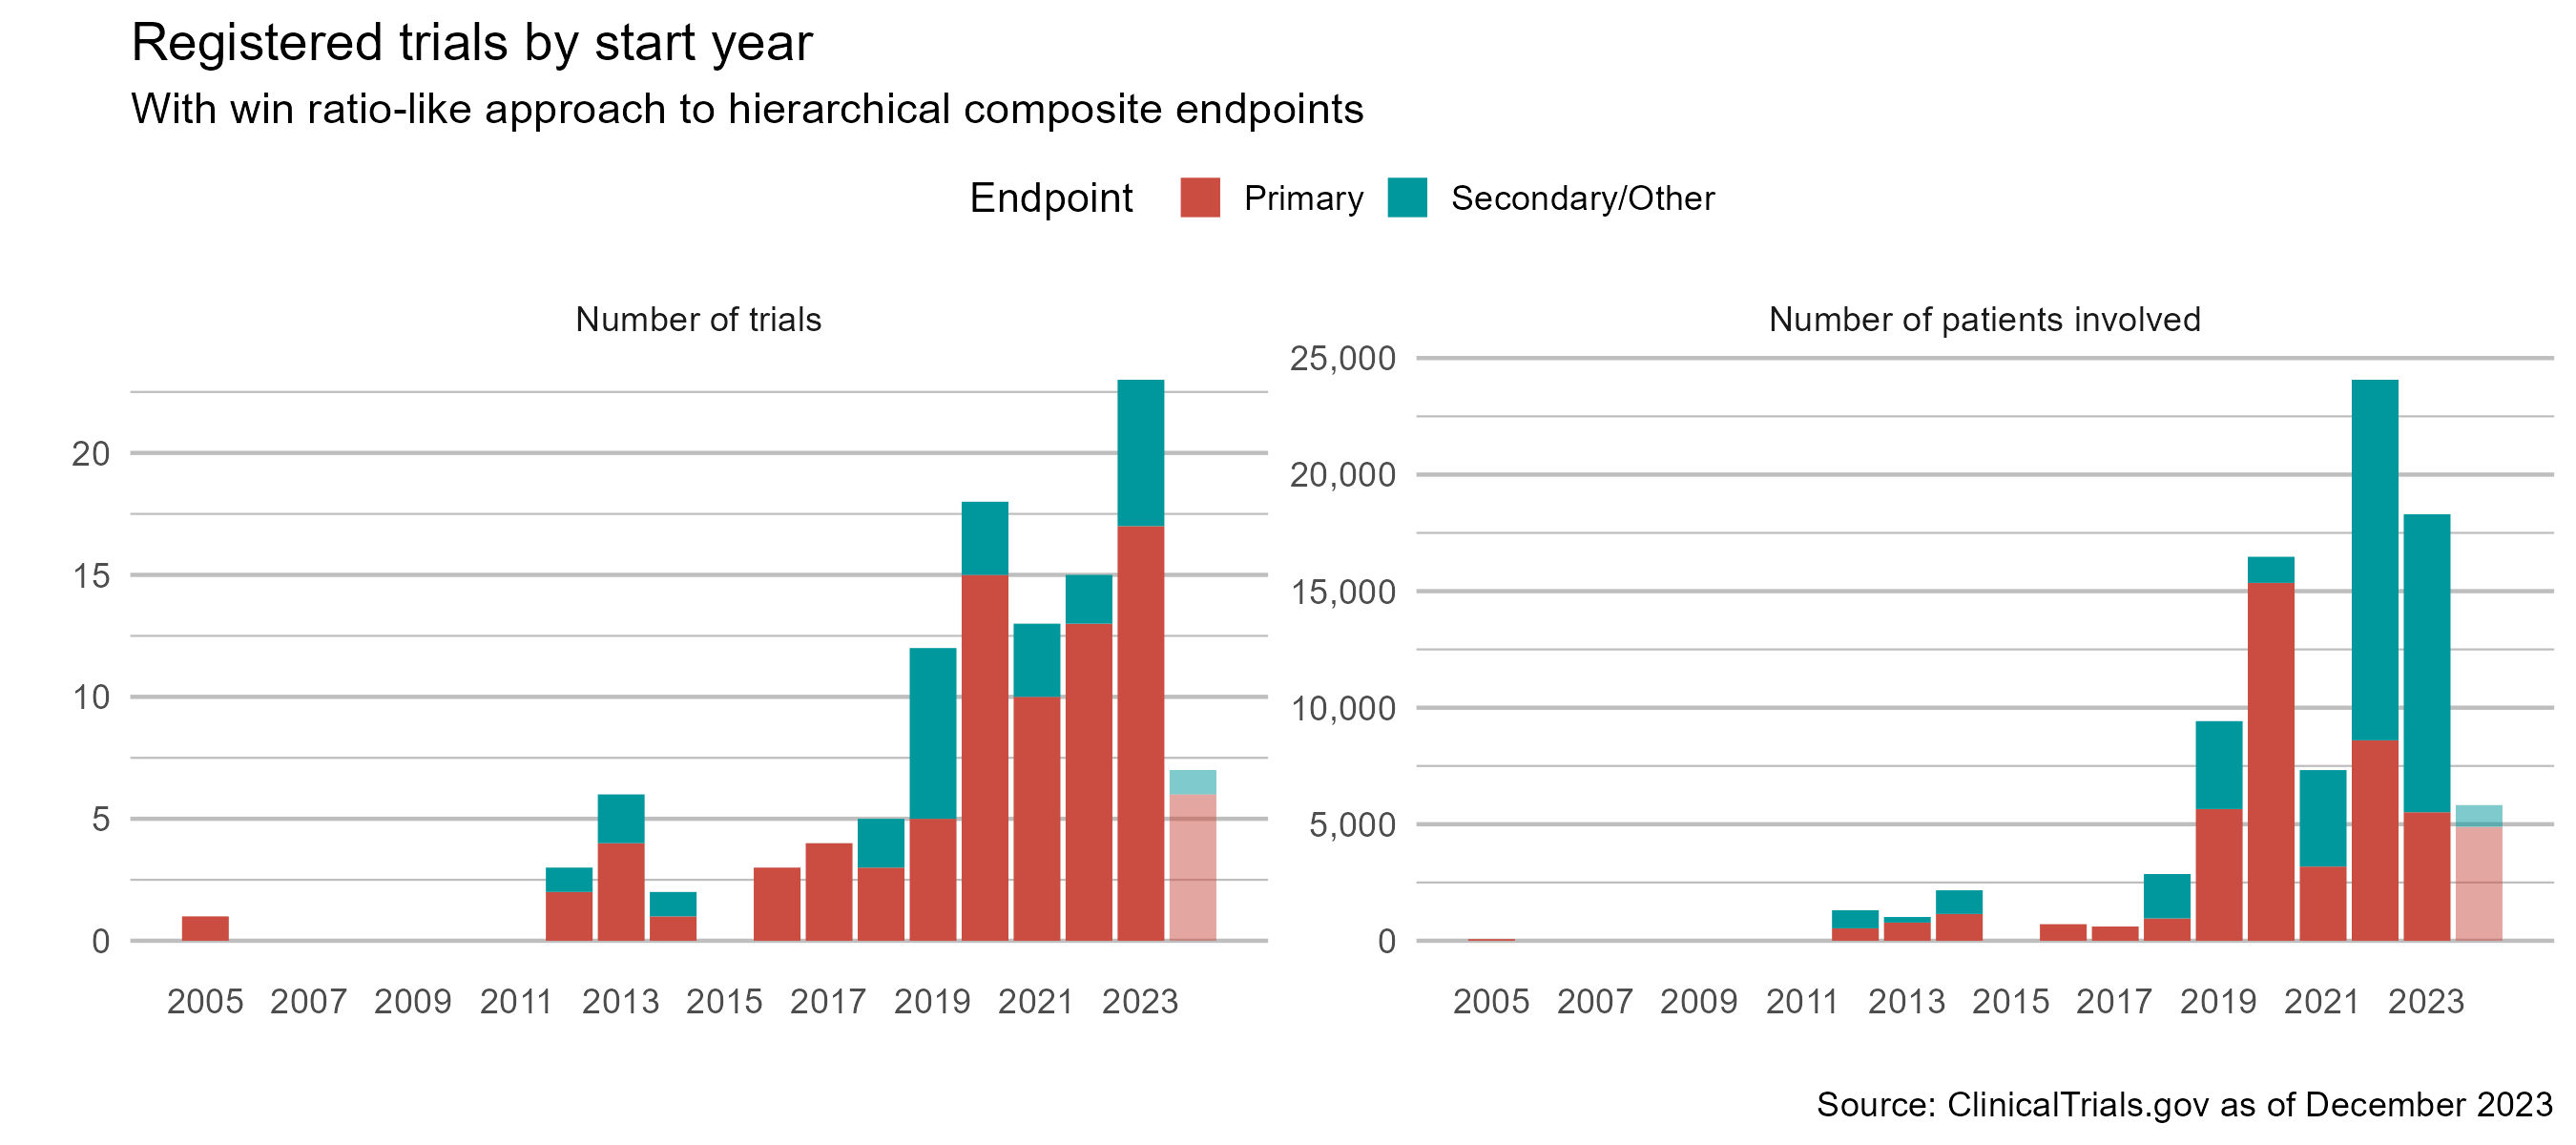
\includegraphics{docs/images/intro_Ntrial_title.png}

\bookmarksetup{startatroot}

\hypertarget{introduction}{%
\chapter{Introduction}\label{introduction}}

\hypertarget{slides}{%
\section*{Slides}\label{slides}}
\addcontentsline{toc}{section}{Slides}

\markright{Slides}

Chapter slides \href{chap1.html}{here}. (To convert html to pdf, press E
\(\to\) Print \(\to\) Destination: Save to pdf)

\hypertarget{r-code}{%
\section*{R-code}\label{r-code}}
\addcontentsline{toc}{section}{R-code}

\markright{R-code}

\begin{Shaded}
\begin{Highlighting}[]
\DocumentationTok{\#\#\#\#\#\#\#\#\#\#\#\#\#\#\#\#\#\#\#\#\#\#\#\#\#\#\#\#\#\#\#\#\#\#\#\#\#\#\#\#\#\#\#\#\#\#\#\#\#\#\#\#\#\#\#\#\#\#\#\#\#\#\#\#\#\#}
\CommentTok{\# This code generates the numerical results in  chapter 1       \#\#}
\DocumentationTok{\#\#\#\#\#\#\#\#\#\#\#\#\#\#\#\#\#\#\#\#\#\#\#\#\#\#\#\#\#\#\#\#\#\#\#\#\#\#\#\#\#\#\#\#\#\#\#\#\#\#\#\#\#\#\#\#\#\#\#\#\#\#\#\#\#\#}

\CommentTok{\# load the survival package}
\FunctionTok{library}\NormalTok{(survival)}
\CommentTok{\# install.packages("Wcompo")}
\FunctionTok{library}\NormalTok{(Wcompo) }\CommentTok{\# for weighted total events}
\FunctionTok{library}\NormalTok{(rmt) }\CommentTok{\# for hfaction data}
\FunctionTok{library}\NormalTok{(tidyverse) }\CommentTok{\# for data wrangling}

\CommentTok{\# load hfaction data}
\FunctionTok{data}\NormalTok{(hfaction)}
\FunctionTok{head}\NormalTok{(hfaction)}

\CommentTok{\# convert status=1 for death, 2=hospitalization}
\NormalTok{hfaction }\OtherTok{\textless{}{-}}\NormalTok{ hfaction }\SpecialCharTok{|\textgreater{}} 
  \FunctionTok{mutate}\NormalTok{(}
    \AttributeTok{status =} \FunctionTok{case\_when}\NormalTok{(}
\NormalTok{      status }\SpecialCharTok{==} \DecValTok{1} \SpecialCharTok{\textasciitilde{}} \DecValTok{2}\NormalTok{,}
\NormalTok{      status }\SpecialCharTok{==} \DecValTok{2} \SpecialCharTok{\textasciitilde{}} \DecValTok{1}\NormalTok{,}
\NormalTok{      status }\SpecialCharTok{==} \DecValTok{0} \SpecialCharTok{\textasciitilde{}} \DecValTok{0}
\NormalTok{    )}
\NormalTok{  )}

\FunctionTok{head}\NormalTok{(hfaction)}

\CommentTok{\# count unique patients in each arm}
\NormalTok{hfaction }\SpecialCharTok{|\textgreater{}} 
  \FunctionTok{group\_by}\NormalTok{(trt\_ab) }\SpecialCharTok{|\textgreater{}} 
  \FunctionTok{distinct}\NormalTok{(patid) }\SpecialCharTok{|\textgreater{}} 
  \FunctionTok{count}\NormalTok{(trt\_ab)}

\CommentTok{\# TFE: take the first event per patient id}
\NormalTok{hfaction\_TFE }\OtherTok{\textless{}{-}}\NormalTok{ hfaction }\SpecialCharTok{|\textgreater{}} 
  \FunctionTok{arrange}\NormalTok{(patid, time) }\SpecialCharTok{|\textgreater{}} 
  \FunctionTok{group\_by}\NormalTok{(patid) }\SpecialCharTok{|\textgreater{}} 
  \FunctionTok{slice\_head}\NormalTok{() }\SpecialCharTok{|\textgreater{}} 
  \FunctionTok{ungroup}\NormalTok{()}

\CommentTok{\# Mortality analysis {-}{-}{-}{-}{-}{-}{-}{-}{-}{-}{-}{-}{-}{-}{-}{-}{-}{-}{-}{-}{-}{-}{-}{-}{-}{-}{-}{-}{-}{-}{-}{-}{-}{-}{-}{-}{-}{-}{-}{-}{-}{-}{-}{-}{-}{-}{-}{-}{-}{-}{-}{-}{-}{-}}

\DocumentationTok{\#\# get mortality data}
\NormalTok{hfaction\_D }\OtherTok{\textless{}{-}}\NormalTok{ hfaction }\SpecialCharTok{|\textgreater{}} 
  \FunctionTok{filter}\NormalTok{(status }\SpecialCharTok{!=} \DecValTok{2}\NormalTok{) }\CommentTok{\# remove hospitalization records}

\DocumentationTok{\#\# Cox model for death against trt\_ab}
\NormalTok{obj\_D }\OtherTok{\textless{}{-}} \FunctionTok{coxph}\NormalTok{(}\FunctionTok{Surv}\NormalTok{(time, status) }\SpecialCharTok{\textasciitilde{}}\NormalTok{ trt\_ab, }\AttributeTok{data =}\NormalTok{ hfaction\_D)}
\FunctionTok{summary}\NormalTok{(obj\_D)}
\CommentTok{\#\textgreater{} n= 426, number of events= 93 }
\CommentTok{\#\textgreater{} coef exp(coef) se(coef)      z Pr(\textgreater{}|z|)  }
\CommentTok{\#\textgreater{} trt\_ab {-}0.3973    0.6721   0.2129 {-}1.866   0.0621 .}

\CommentTok{\# TFE analysis {-}{-}{-}{-}{-}{-}{-}{-}{-}{-}{-}{-}{-}{-}{-}{-}{-}{-}{-}{-}{-}{-}{-}{-}{-}{-}{-}{-}{-}{-}{-}{-}{-}{-}{-}{-}{-}{-}{-}{-}{-}{-}{-}{-}{-}{-}{-}{-}{-}{-}{-}{-}{-}{-}{-}{-}}

\DocumentationTok{\#\# how many of first events are death (1) or hosp (2)}
\NormalTok{hfaction\_TFE }\SpecialCharTok{|\textgreater{}} 
  \FunctionTok{count}\NormalTok{(status)}

\CommentTok{\# Cox model for TFE against trt\_ab}
\NormalTok{obj\_TFE }\OtherTok{\textless{}{-}} \FunctionTok{coxph}\NormalTok{(}\FunctionTok{Surv}\NormalTok{(time, status }\SpecialCharTok{\textgreater{}} \DecValTok{0}\NormalTok{) }\SpecialCharTok{\textasciitilde{}}\NormalTok{ trt\_ab, }\AttributeTok{data =}\NormalTok{ hfaction\_TFE)}
\FunctionTok{summary}\NormalTok{(obj\_TFE)}


\CommentTok{\# Mortality vs TFE {-}{-}{-}{-}{-}{-}{-}{-}{-}{-}{-}{-}{-}{-}{-}{-}{-}{-}{-}{-}{-}{-}{-}{-}{-}{-}{-}{-}{-}{-}{-}{-}{-}{-}{-}{-}{-}{-}{-}{-}{-}{-}{-}{-}{-}{-}{-}{-}{-}{-}{-}{-}{-}{-}{-}{-}}

\FunctionTok{library}\NormalTok{(ggsurvfit)}
\FunctionTok{library}\NormalTok{(patchwork)}

\NormalTok{pD }\OtherTok{\textless{}{-}} \FunctionTok{survfit2}\NormalTok{(}\FunctionTok{Surv}\NormalTok{(time, status) }\SpecialCharTok{\textasciitilde{}}\NormalTok{ trt\_ab, }\AttributeTok{data =}\NormalTok{ hfaction\_D) }\SpecialCharTok{|\textgreater{}}
  \FunctionTok{ggsurvfit}\NormalTok{(}\AttributeTok{linewidth =} \DecValTok{1}\NormalTok{) }\SpecialCharTok{+}
  \FunctionTok{scale\_ggsurvfit}\NormalTok{() }\SpecialCharTok{+}
  \FunctionTok{scale\_color\_discrete}\NormalTok{(}\AttributeTok{labels =} \FunctionTok{c}\NormalTok{(}\StringTok{"Usual care"}\NormalTok{, }\StringTok{"Training"}\NormalTok{)) }\SpecialCharTok{+}
  \FunctionTok{scale\_x\_continuous}\NormalTok{(}\StringTok{"Time (years)"}\NormalTok{, }\AttributeTok{limits =} \FunctionTok{c}\NormalTok{(}\DecValTok{0}\NormalTok{, }\DecValTok{4}\NormalTok{)) }\SpecialCharTok{+}
  \FunctionTok{labs}\NormalTok{(}\AttributeTok{y =} \StringTok{"Overall survival"}\NormalTok{)}

\NormalTok{pTFE }\OtherTok{\textless{}{-}} \FunctionTok{survfit2}\NormalTok{(}\FunctionTok{Surv}\NormalTok{(time, status }\SpecialCharTok{\textgreater{}} \DecValTok{0}\NormalTok{) }\SpecialCharTok{\textasciitilde{}}\NormalTok{ trt\_ab, }\AttributeTok{data =}\NormalTok{ hfaction\_TFE) }\SpecialCharTok{|\textgreater{}}
  \FunctionTok{ggsurvfit}\NormalTok{(}\AttributeTok{linewidth =} \DecValTok{1}\NormalTok{) }\SpecialCharTok{+}
  \FunctionTok{scale\_ggsurvfit}\NormalTok{() }\SpecialCharTok{+}
  \FunctionTok{scale\_color\_discrete}\NormalTok{(}\AttributeTok{labels =} \FunctionTok{c}\NormalTok{(}\StringTok{"Usual care"}\NormalTok{, }\StringTok{"Training"}\NormalTok{)) }\SpecialCharTok{+}
  \FunctionTok{scale\_x\_continuous}\NormalTok{(}\StringTok{"Time (years)"}\NormalTok{, }\AttributeTok{limits =} \FunctionTok{c}\NormalTok{(}\DecValTok{0}\NormalTok{, }\DecValTok{4}\NormalTok{)) }\SpecialCharTok{+}
  \FunctionTok{labs}\NormalTok{(}\AttributeTok{y =} \StringTok{"Hospitalization{-}free survival"}\NormalTok{)}


\NormalTok{pD }\SpecialCharTok{+}\NormalTok{ pTFE }\SpecialCharTok{+} \FunctionTok{plot\_layout}\NormalTok{(}\AttributeTok{guides =} \StringTok{"collect"}\NormalTok{) }\SpecialCharTok{\&} 
  \FunctionTok{theme}\NormalTok{(}
    \AttributeTok{legend.position =} \StringTok{"top"}\NormalTok{, }
    \AttributeTok{legend.text =} \FunctionTok{element\_text}\NormalTok{(}\AttributeTok{size =} \DecValTok{12}\NormalTok{)}
\NormalTok{    )}

\FunctionTok{ggsave}\NormalTok{(}\StringTok{"images/intro\_hfaction\_unis.png"}\NormalTok{, }\AttributeTok{width =} \DecValTok{8}\NormalTok{, }\AttributeTok{height =} \FloatTok{4.5}\NormalTok{)}

\CommentTok{\# Total events (proportional mean) {-}{-}{-}{-}{-}{-}{-}{-}{-}{-}{-}{-}{-}{-}{-}{-}{-}{-}{-}{-}{-}{-}{-}{-}{-}{-}{-}{-}{-}{-}{-}{-}{-}{-}{-}{-}{-}{-}{-}{-}}
\DocumentationTok{\#\# fit proportional means model with death = 2 x hosp}
\NormalTok{obj\_ML }\OtherTok{\textless{}{-}} \FunctionTok{CompoML}\NormalTok{(hfaction}\SpecialCharTok{$}\NormalTok{patid, hfaction}\SpecialCharTok{$}\NormalTok{time, hfaction}\SpecialCharTok{$}\NormalTok{status, }
\NormalTok{                  hfaction}\SpecialCharTok{$}\NormalTok{trt\_ab, }\AttributeTok{w =} \FunctionTok{c}\NormalTok{(}\DecValTok{2}\NormalTok{, }\DecValTok{1}\NormalTok{))}
\DocumentationTok{\#\# summary results}
\NormalTok{obj\_ML}

\DocumentationTok{\#\# plot model{-}based mean functions}
\FunctionTok{plot}\NormalTok{(obj\_ML, }\DecValTok{0}\NormalTok{, }\AttributeTok{ylim=} \FunctionTok{c}\NormalTok{(}\DecValTok{0}\NormalTok{, }\DecValTok{5}\NormalTok{), }\AttributeTok{xlim=} \FunctionTok{c}\NormalTok{(}\DecValTok{0}\NormalTok{, }\DecValTok{4}\NormalTok{), }\AttributeTok{xlab=}\StringTok{"Time (years)"}\NormalTok{, }
     \AttributeTok{col =} \StringTok{"red"}\NormalTok{, }\AttributeTok{lwd =} \DecValTok{2}\NormalTok{)}
\FunctionTok{plot}\NormalTok{(obj\_ML, }\DecValTok{1}\NormalTok{, }\AttributeTok{add =} \ConstantTok{TRUE}\NormalTok{, }\AttributeTok{col =} \StringTok{"blue"}\NormalTok{, }\AttributeTok{lwd=}\DecValTok{2}\NormalTok{)}
\FunctionTok{legend}\NormalTok{(}\DecValTok{0}\NormalTok{, }\DecValTok{5}\NormalTok{, }\AttributeTok{col =} \FunctionTok{c}\NormalTok{(}\StringTok{"red"}\NormalTok{, }\StringTok{"blue"}\NormalTok{), }\FunctionTok{c}\NormalTok{(}\StringTok{"Usual care"}\NormalTok{,}\StringTok{"Training"}\NormalTok{), }\AttributeTok{lwd =} \DecValTok{2}\NormalTok{)}
\end{Highlighting}
\end{Shaded}

\bookmarksetup{startatroot}

\hypertarget{hypothesis-testing}{%
\chapter{Hypothesis Testing}\label{hypothesis-testing}}

\hypertarget{slides-1}{%
\section*{Slides}\label{slides-1}}
\addcontentsline{toc}{section}{Slides}

\markright{Slides}

Chapter slides \href{chap2.html}{here}. (To convert html to pdf, press E
\(\to\) Print \(\to\) Destination: Save to pdf)

\hypertarget{r-code-1}{%
\section*{R-code}\label{r-code-1}}
\addcontentsline{toc}{section}{R-code}

\markright{R-code}

\begin{Shaded}
\begin{Highlighting}[]
\DocumentationTok{\#\#\#\#\#\#\#\#\#\#\#\#\#\#\#\#\#\#\#\#\#\#\#\#\#\#\#\#\#\#\#\#\#\#\#\#\#\#\#\#\#\#\#\#\#\#\#\#\#\#\#\#\#\#\#\#\#\#\#\#\#\#\#\#\#\#}
\CommentTok{\# This code generates the numerical results in  chapter 2       \#\#}
\DocumentationTok{\#\#\#\#\#\#\#\#\#\#\#\#\#\#\#\#\#\#\#\#\#\#\#\#\#\#\#\#\#\#\#\#\#\#\#\#\#\#\#\#\#\#\#\#\#\#\#\#\#\#\#\#\#\#\#\#\#\#\#\#\#\#\#\#\#\#}


\CommentTok{\# load the survival package}
\FunctionTok{library}\NormalTok{(survival)}

\CommentTok{\# install and load the WR package for}
\CommentTok{\# 1. dataset hfaction\_cpx9;}
\CommentTok{\# 2. function WRrec() for win ratio test (of recurrent events and death)}
\CommentTok{\# 3. functions base() and WRSS() for sample size calculation}
\CommentTok{\# install.packages("WR")}
\FunctionTok{library}\NormalTok{(WR)}
\FunctionTok{library}\NormalTok{(tidyverse) }\CommentTok{\# for data wrangling}


\DocumentationTok{\#\#\#\#\# Read in HF{-}ACTION DATA\#\#\#\#\#\#\#\#}
\CommentTok{\# same as rmt::hfaction used in chap 1 }
\CommentTok{\#  (except for status coding)}
\FunctionTok{data}\NormalTok{(hfaction\_cpx9)}
\NormalTok{hfaction }\OtherTok{\textless{}{-}}\NormalTok{ hfaction\_cpx9}
\FunctionTok{head}\NormalTok{(hfaction)}


\CommentTok{\# count unique patients in each arm}
\NormalTok{hfaction }\SpecialCharTok{|\textgreater{}} 
  \FunctionTok{group\_by}\NormalTok{(trt\_ab) }\SpecialCharTok{|\textgreater{}} 
  \FunctionTok{distinct}\NormalTok{(patid) }\SpecialCharTok{|\textgreater{}} 
  \FunctionTok{count}\NormalTok{(trt\_ab)}
  
\DocumentationTok{\#\#\#\# demo \#\#\#\#\#\#\#\#\#\#\#\#}
\NormalTok{obj }\OtherTok{\textless{}{-}} \FunctionTok{WRrec}\NormalTok{(}\AttributeTok{ID =}\NormalTok{ hfaction}\SpecialCharTok{$}\NormalTok{patid, }\AttributeTok{time =}\NormalTok{ hfaction}\SpecialCharTok{$}\NormalTok{time, }
             \AttributeTok{status =}\NormalTok{ hfaction}\SpecialCharTok{$}\NormalTok{status, }\AttributeTok{trt =}\NormalTok{ hfaction}\SpecialCharTok{$}\NormalTok{trt\_ab,}
             \AttributeTok{strata =}\NormalTok{ hfaction}\SpecialCharTok{$}\NormalTok{age60, }\AttributeTok{naive =} \ConstantTok{TRUE}\NormalTok{)}
\CommentTok{\# summary results}
\NormalTok{obj}

\CommentTok{\# LWR}
\NormalTok{beta }\OtherTok{\textless{}{-}}\NormalTok{ obj}\SpecialCharTok{$}\NormalTok{log.WR}
\NormalTok{se }\OtherTok{\textless{}{-}}\NormalTok{ obj}\SpecialCharTok{$}\NormalTok{se}
\CommentTok{\# test}
\NormalTok{pval }\OtherTok{\textless{}{-}} \DecValTok{2}\SpecialCharTok{*}\NormalTok{(}\DecValTok{1}\SpecialCharTok{{-}}\FunctionTok{pnorm}\NormalTok{(}\FunctionTok{abs}\NormalTok{(beta}\SpecialCharTok{/}\NormalTok{se)))}
\NormalTok{pval}

\CommentTok{\# NWR}
\NormalTok{beta.naive}\OtherTok{\textless{}{-}}\NormalTok{obj}\SpecialCharTok{$}\NormalTok{log.WR.naive}
\NormalTok{se.naive}\OtherTok{\textless{}{-}}\NormalTok{obj}\SpecialCharTok{$}\NormalTok{se.naive}
\CommentTok{\# test}
\NormalTok{pval.naive}\OtherTok{\textless{}{-}}\DecValTok{2}\SpecialCharTok{*}\NormalTok{(}\DecValTok{1}\SpecialCharTok{{-}}\FunctionTok{pnorm}\NormalTok{(}\FunctionTok{abs}\NormalTok{(beta.naive}\SpecialCharTok{/}\NormalTok{se.naive)))}
\NormalTok{pval.naive}


\CommentTok{\# FWR}
\NormalTok{beta.FI}\OtherTok{\textless{}{-}}\NormalTok{obj}\SpecialCharTok{$}\NormalTok{log.WR.FI}
\NormalTok{se.FI}\OtherTok{\textless{}{-}}\NormalTok{obj}\SpecialCharTok{$}\NormalTok{se.FI}
\CommentTok{\# test}
\NormalTok{pval.FI}\OtherTok{\textless{}{-}}\DecValTok{2}\SpecialCharTok{*}\NormalTok{(}\DecValTok{1}\SpecialCharTok{{-}}\FunctionTok{pnorm}\NormalTok{(}\FunctionTok{abs}\NormalTok{(beta.FI}\SpecialCharTok{/}\NormalTok{se.FI)))}
\NormalTok{pval.FI}


\DocumentationTok{\#\#\#\#\#\#\#\#\#\#\#\#\#\#\#\#\#\#\#\#\#\#\#\#\#\#\#\#\#\#\#\#\#}
\CommentTok{\# Win ratio analyses: tabulate  \#}
\DocumentationTok{\#\#\#\#\#\#\#\#\#\#\#\#\#\#\#\#\#\#\#\#\#\#\#\#\#\#\#\#\#\#\#\#\#}

\NormalTok{data }\OtherTok{\textless{}{-}}\NormalTok{ hfaction }
\DocumentationTok{\#\#\# create a dataset with only the first hospitalization data.H1}

\CommentTok{\# hospitalization data}
\NormalTok{tmpH }\OtherTok{\textless{}{-}}\NormalTok{ data[data}\SpecialCharTok{$}\NormalTok{status}\SpecialCharTok{==}\DecValTok{2}\NormalTok{,]}
\CommentTok{\# get the first record of each id}
\NormalTok{o }\OtherTok{\textless{}{-}} \FunctionTok{order}\NormalTok{(tmpH}\SpecialCharTok{$}\NormalTok{patid,tmpH}\SpecialCharTok{$}\NormalTok{time)}
\NormalTok{tmpH }\OtherTok{\textless{}{-}}\NormalTok{ tmpH[o,]}
\NormalTok{tmpFH }\OtherTok{\textless{}{-}}\NormalTok{ tmpH[}\SpecialCharTok{!}\FunctionTok{duplicated}\NormalTok{(tmpH}\SpecialCharTok{$}\NormalTok{patid),]}

\CommentTok{\# combine it with mortality data}
\NormalTok{data.H1 }\OtherTok{\textless{}{-}} \FunctionTok{rbind}\NormalTok{(tmpFH,data[data}\SpecialCharTok{$}\NormalTok{status}\SpecialCharTok{!=}\DecValTok{2}\NormalTok{,])}
\NormalTok{o }\OtherTok{\textless{}{-}} \FunctionTok{order}\NormalTok{(data.H1}\SpecialCharTok{$}\NormalTok{patid,data.H1}\SpecialCharTok{$}\NormalTok{time)}
\NormalTok{data.H1 }\OtherTok{\textless{}{-}}\NormalTok{ data.H1[o,]}


\CommentTok{\# Function to create table for estimates of }
\CommentTok{\# PWR, NWR, FWR, and LWR, 95\% CI nad p{-}values}
\CommentTok{\# ind: index for data}
\CommentTok{\# ind1: index for data.H1}
\CommentTok{\# r: number of decimal point}
\NormalTok{gwr.fun}\OtherTok{=}\ControlFlowTok{function}\NormalTok{(ind,ind1,}\AttributeTok{r=}\DecValTok{2}\NormalTok{)\{}

\CommentTok{\# fit NWR, FWR, and LWR}
\NormalTok{obj }\OtherTok{\textless{}{-}} \FunctionTok{WRrec}\NormalTok{(}\AttributeTok{ID=}\NormalTok{data}\SpecialCharTok{$}\NormalTok{patid[ind],}\AttributeTok{time=}\NormalTok{data}\SpecialCharTok{$}\NormalTok{time[ind],}\AttributeTok{status=}\NormalTok{data}\SpecialCharTok{$}\NormalTok{status[ind],}
          \AttributeTok{trt=}\NormalTok{data}\SpecialCharTok{$}\NormalTok{trt\_ab[ind],}\AttributeTok{strata=}\NormalTok{data}\SpecialCharTok{$}\NormalTok{age60[ind],}\AttributeTok{naive=}\NormalTok{T)}
\CommentTok{\# fit sWR}
\NormalTok{obj1 }\OtherTok{\textless{}{-}} \FunctionTok{WRrec}\NormalTok{(}\AttributeTok{ID=}\NormalTok{data.H1}\SpecialCharTok{$}\NormalTok{patid[ind1],}\AttributeTok{time=}\NormalTok{data.H1}\SpecialCharTok{$}\NormalTok{time[ind1],}\AttributeTok{status=}\NormalTok{data.H1}\SpecialCharTok{$}\NormalTok{status[ind1],}
          \AttributeTok{trt=}\NormalTok{data.H1}\SpecialCharTok{$}\NormalTok{trt\_ab[ind1],}\AttributeTok{strata=}\NormalTok{data.H1}\SpecialCharTok{$}\NormalTok{age60[ind1],}\AttributeTok{naive=}\NormalTok{F)}

\CommentTok{\# critical value of p=0.05}
\NormalTok{za }\OtherTok{\textless{}{-}} \FunctionTok{qnorm}\NormalTok{(}\FloatTok{0.975}\NormalTok{)}

\DocumentationTok{\#\# LWR}
\NormalTok{beta }\OtherTok{\textless{}{-}}\NormalTok{ obj}\SpecialCharTok{$}\NormalTok{log.WR}
\NormalTok{se }\OtherTok{\textless{}{-}}\NormalTok{ obj}\SpecialCharTok{$}\NormalTok{se}
\NormalTok{theta }\OtherTok{\textless{}{-}}\NormalTok{ obj}\SpecialCharTok{$}\NormalTok{theta}

\NormalTok{r4 }\OtherTok{\textless{}{-}} \FunctionTok{c}\NormalTok{(}\FunctionTok{paste0}\NormalTok{(}\FunctionTok{round}\NormalTok{(}\DecValTok{100}\SpecialCharTok{*}\NormalTok{theta[}\DecValTok{1}\NormalTok{],}\DecValTok{1}\NormalTok{),}\StringTok{"\%"}\NormalTok{),}
     \FunctionTok{paste0}\NormalTok{(}\FunctionTok{round}\NormalTok{(}\DecValTok{100}\SpecialCharTok{*}\NormalTok{theta[}\DecValTok{2}\NormalTok{],}\DecValTok{1}\NormalTok{),}\StringTok{"\%"}\NormalTok{),}
     \FunctionTok{paste0}\NormalTok{(}\FunctionTok{round}\NormalTok{(}\FunctionTok{exp}\NormalTok{(beta),r),}\StringTok{" ("}\NormalTok{,}\FunctionTok{round}\NormalTok{(}\FunctionTok{exp}\NormalTok{(beta}\SpecialCharTok{{-}}\NormalTok{za}\SpecialCharTok{*}\NormalTok{se),r),}\StringTok{", "}\NormalTok{,}\FunctionTok{round}\NormalTok{(}\FunctionTok{exp}\NormalTok{(beta}\SpecialCharTok{+}\NormalTok{za}\SpecialCharTok{*}\NormalTok{se),r),}\StringTok{")"}\NormalTok{),}
     \FunctionTok{round}\NormalTok{(}\DecValTok{1}\SpecialCharTok{{-}}\FunctionTok{pchisq}\NormalTok{((beta}\SpecialCharTok{/}\NormalTok{se)}\SpecialCharTok{\^{}}\DecValTok{2}\NormalTok{,}\DecValTok{1}\NormalTok{),}\DecValTok{3}\NormalTok{)}
\NormalTok{)}


\DocumentationTok{\#\# PWR}
\NormalTok{beta1}\OtherTok{=}\NormalTok{obj1}\SpecialCharTok{$}\NormalTok{log.WR}
\NormalTok{se1}\OtherTok{=}\NormalTok{obj1}\SpecialCharTok{$}\NormalTok{se}
\NormalTok{theta1}\OtherTok{=}\NormalTok{obj1}\SpecialCharTok{$}\NormalTok{theta}

\NormalTok{r1}\OtherTok{=}\FunctionTok{c}\NormalTok{(}\FunctionTok{paste0}\NormalTok{(}\FunctionTok{round}\NormalTok{(}\DecValTok{100}\SpecialCharTok{*}\NormalTok{theta1[}\DecValTok{1}\NormalTok{],}\DecValTok{1}\NormalTok{),}\StringTok{"\%"}\NormalTok{),}
     \FunctionTok{paste0}\NormalTok{(}\FunctionTok{round}\NormalTok{(}\DecValTok{100}\SpecialCharTok{*}\NormalTok{theta1[}\DecValTok{2}\NormalTok{],}\DecValTok{1}\NormalTok{),}\StringTok{"\%"}\NormalTok{),}
     \FunctionTok{paste0}\NormalTok{(}\FunctionTok{round}\NormalTok{(}\FunctionTok{exp}\NormalTok{(beta1),r),}\StringTok{" ("}\NormalTok{,}\FunctionTok{round}\NormalTok{(}\FunctionTok{exp}\NormalTok{(beta1}\SpecialCharTok{{-}}\NormalTok{za}\SpecialCharTok{*}\NormalTok{se1),r),}\StringTok{", "}\NormalTok{,}\FunctionTok{round}\NormalTok{(}\FunctionTok{exp}\NormalTok{(beta1}\SpecialCharTok{+}\NormalTok{za}\SpecialCharTok{*}\NormalTok{se1),r),}\StringTok{")"}\NormalTok{),}
     \FunctionTok{round}\NormalTok{(}\DecValTok{1}\SpecialCharTok{{-}}\FunctionTok{pchisq}\NormalTok{((beta1}\SpecialCharTok{/}\NormalTok{se1)}\SpecialCharTok{\^{}}\DecValTok{2}\NormalTok{,}\DecValTok{1}\NormalTok{),}\DecValTok{3}\NormalTok{)}
\NormalTok{)}

\DocumentationTok{\#\# NWR}
\NormalTok{beta.naive}\OtherTok{=}\NormalTok{obj}\SpecialCharTok{$}\NormalTok{log.WR.naive}
\NormalTok{se.naive}\OtherTok{=}\NormalTok{obj}\SpecialCharTok{$}\NormalTok{se.naive}
\NormalTok{theta.naive}\OtherTok{=}\NormalTok{obj}\SpecialCharTok{$}\NormalTok{theta.naive}


\NormalTok{r2}\OtherTok{=}\FunctionTok{c}\NormalTok{(}\FunctionTok{paste0}\NormalTok{(}\FunctionTok{round}\NormalTok{(}\DecValTok{100}\SpecialCharTok{*}\NormalTok{theta.naive[}\DecValTok{1}\NormalTok{],}\DecValTok{1}\NormalTok{),}\StringTok{"\%"}\NormalTok{),}
     \FunctionTok{paste0}\NormalTok{(}\FunctionTok{round}\NormalTok{(}\DecValTok{100}\SpecialCharTok{*}\NormalTok{theta.naive[}\DecValTok{2}\NormalTok{],}\DecValTok{1}\NormalTok{),}\StringTok{"\%"}\NormalTok{),}
     \FunctionTok{paste0}\NormalTok{(}\FunctionTok{round}\NormalTok{(}\FunctionTok{exp}\NormalTok{(beta.naive),r),}\StringTok{" ("}\NormalTok{,}\FunctionTok{round}\NormalTok{(}\FunctionTok{exp}\NormalTok{(beta.naive}\SpecialCharTok{{-}}\NormalTok{za}\SpecialCharTok{*}\NormalTok{se.naive),r),}\StringTok{", "}\NormalTok{,}
            \FunctionTok{round}\NormalTok{(}\FunctionTok{exp}\NormalTok{(beta.naive}\SpecialCharTok{+}\NormalTok{za}\SpecialCharTok{*}\NormalTok{se.naive),r),}\StringTok{")"}\NormalTok{),}
     \FunctionTok{round}\NormalTok{(}\DecValTok{1}\SpecialCharTok{{-}}\FunctionTok{pchisq}\NormalTok{((beta.naive}\SpecialCharTok{/}\NormalTok{se.naive)}\SpecialCharTok{\^{}}\DecValTok{2}\NormalTok{,}\DecValTok{1}\NormalTok{),}\DecValTok{3}\NormalTok{)}
\NormalTok{)}




\DocumentationTok{\#\# FWR}
\NormalTok{beta.FI}\OtherTok{=}\NormalTok{obj}\SpecialCharTok{$}\NormalTok{log.WR.FI}
\NormalTok{se.FI}\OtherTok{=}\NormalTok{obj}\SpecialCharTok{$}\NormalTok{se.FI}
\NormalTok{theta.FI}\OtherTok{=}\NormalTok{obj}\SpecialCharTok{$}\NormalTok{theta.FI}


\NormalTok{r3}\OtherTok{=}\FunctionTok{c}\NormalTok{(}\FunctionTok{paste0}\NormalTok{(}\FunctionTok{round}\NormalTok{(}\DecValTok{100}\SpecialCharTok{*}\NormalTok{theta.FI[}\DecValTok{1}\NormalTok{],}\DecValTok{1}\NormalTok{),}\StringTok{"\%"}\NormalTok{),}
     \FunctionTok{paste0}\NormalTok{(}\FunctionTok{round}\NormalTok{(}\DecValTok{100}\SpecialCharTok{*}\NormalTok{theta.FI[}\DecValTok{2}\NormalTok{],}\DecValTok{1}\NormalTok{),}\StringTok{"\%"}\NormalTok{),}
     \FunctionTok{paste0}\NormalTok{(}\FunctionTok{round}\NormalTok{(}\FunctionTok{exp}\NormalTok{(beta.FI),r),}\StringTok{" ("}\NormalTok{,}\FunctionTok{round}\NormalTok{(}\FunctionTok{exp}\NormalTok{(beta.FI}\SpecialCharTok{{-}}\NormalTok{za}\SpecialCharTok{*}\NormalTok{se.FI),r),}\StringTok{", "}\NormalTok{,}
            \FunctionTok{round}\NormalTok{(}\FunctionTok{exp}\NormalTok{(beta.FI}\SpecialCharTok{+}\NormalTok{za}\SpecialCharTok{*}\NormalTok{se.FI),r),}\StringTok{")"}\NormalTok{),}
     \FunctionTok{round}\NormalTok{(}\DecValTok{1}\SpecialCharTok{{-}}\FunctionTok{pchisq}\NormalTok{((beta.FI}\SpecialCharTok{/}\NormalTok{se.FI)}\SpecialCharTok{\^{}}\DecValTok{2}\NormalTok{,}\DecValTok{1}\NormalTok{),}\DecValTok{3}\NormalTok{)}
\NormalTok{)}

\NormalTok{result}\OtherTok{=}\FunctionTok{rbind}\NormalTok{(r1,r2,r3,r4)}
\FunctionTok{rownames}\NormalTok{(result)}\OtherTok{=}\FunctionTok{c}\NormalTok{(}\StringTok{"PWR"}\NormalTok{,}\StringTok{"NWR"}\NormalTok{,}\StringTok{"FWR"}\NormalTok{,}\StringTok{"LWR"}\NormalTok{)}

\FunctionTok{return}\NormalTok{(result)}
\NormalTok{\}}


\CommentTok{\# Create table}
\DocumentationTok{\#\# Age \textless{}= 60 years}
\NormalTok{ind}\OtherTok{=}\NormalTok{(data}\SpecialCharTok{$}\NormalTok{age60}\SpecialCharTok{==}\DecValTok{0}\NormalTok{)}
\NormalTok{ind1}\OtherTok{=}\NormalTok{(data.H1}\SpecialCharTok{$}\NormalTok{age60}\SpecialCharTok{==}\DecValTok{0}\NormalTok{)}
\NormalTok{result.lt60}\OtherTok{=}\FunctionTok{gwr.fun}\NormalTok{(ind,ind1,}\AttributeTok{r=}\DecValTok{2}\NormalTok{)}

\DocumentationTok{\#\# Age \textgreater{} 60 years}
\NormalTok{ind}\OtherTok{=}\NormalTok{(data}\SpecialCharTok{$}\NormalTok{age60}\SpecialCharTok{==}\DecValTok{1}\NormalTok{)}
\NormalTok{ind1}\OtherTok{=}\NormalTok{(data.H1}\SpecialCharTok{$}\NormalTok{age60}\SpecialCharTok{==}\DecValTok{1}\NormalTok{)}
\NormalTok{result.ge60}\OtherTok{=}\FunctionTok{gwr.fun}\NormalTok{(ind,ind1,}\AttributeTok{r=}\DecValTok{2}\NormalTok{)}

\DocumentationTok{\#\# overall}
\NormalTok{ind}\OtherTok{=}\FunctionTok{rep}\NormalTok{(T,}\FunctionTok{nrow}\NormalTok{(data))}
\NormalTok{ind1}\OtherTok{=}\FunctionTok{rep}\NormalTok{(T,}\FunctionTok{nrow}\NormalTok{(data.H1))}
\NormalTok{result.all}\OtherTok{=}\FunctionTok{gwr.fun}\NormalTok{(ind,ind1,}\AttributeTok{r=}\DecValTok{2}\NormalTok{)}

\CommentTok{\# combine results }
\NormalTok{results}\OtherTok{=}\FunctionTok{rbind}\NormalTok{(result.lt60,result.ge60,result.all)}
\FunctionTok{colnames}\NormalTok{(results)}\OtherTok{=}\FunctionTok{c}\NormalTok{(}\StringTok{"Win"}\NormalTok{, }\StringTok{"Loss"}\NormalTok{, }\StringTok{"Win ratio (95\% CI)"}\NormalTok{, }\StringTok{"p{-}value"}\NormalTok{)}
\FunctionTok{noquote}\NormalTok{(results)}



\DocumentationTok{\#\#\#\#\#\#\#\#\#\#\#\#\#\#\#\#\#\#\#\#\#\#\#\#\#\#\#\#\#\#\#\#\#\#\#\#\#\#\#\#\#\#\#\#\#\#\#\#\#\#\#\#\#\#\#\#\#\#\#\#\#\#\#\#\#\#\#\#\#\#\#\#\#\#\#\#}
\CommentTok{\#               Sample size calculation                                    \#     }
\DocumentationTok{\#\#\#\#\#\#\#\#\#\#\#\#\#\#\#\#\#\#\#\#\#\#\#\#\#\#\#\#\#\#\#\#\#\#\#\#\#\#\#\#\#\#\#\#\#\#\#\#\#\#\#\#\#\#\#\#\#\#\#\#\#\#\#\#\#\#\#\#\#\#\#\#\#\#\#\#}

\CommentTok{\# get training arm data}
\NormalTok{pilot }\OtherTok{\textless{}{-}}\NormalTok{ hfaction }\SpecialCharTok{|\textgreater{}} 
  \FunctionTok{filter}\NormalTok{(trt\_ab }\SpecialCharTok{==} \DecValTok{1}\NormalTok{)}
\CommentTok{\# number of subjects}
\NormalTok{pilot }\SpecialCharTok{|\textgreater{}} \FunctionTok{distinct}\NormalTok{(patid) }\SpecialCharTok{|\textgreater{}} 
  \FunctionTok{count}\NormalTok{()}

\DocumentationTok{\#\#\#\#\#\#\#\#\#\#\#\#\#\# estimate parameters \#\#\#\#\#\#\#\#\#\#\#\#\#\#}
\CommentTok{\# Get the variables from pilot dataset}
\CommentTok{\# to estimate baseline parameters }
\CommentTok{\# lambda\_D, lambda\_H, kappa}

\NormalTok{outcome\_base }\OtherTok{\textless{}{-}} \FunctionTok{gumbel.est}\NormalTok{(pilot}\SpecialCharTok{$}\NormalTok{patid, pilot}\SpecialCharTok{$}\NormalTok{time }\SpecialCharTok{/} \DecValTok{12}\NormalTok{, pilot}\SpecialCharTok{$}\NormalTok{status)}

\NormalTok{lambda\_D }\OtherTok{\textless{}{-}}\NormalTok{ outcome\_base}\SpecialCharTok{$}\NormalTok{lambda\_D}
\NormalTok{lambda\_H }\OtherTok{\textless{}{-}}\NormalTok{ outcome\_base}\SpecialCharTok{$}\NormalTok{lambda\_H}
\NormalTok{kappa }\OtherTok{\textless{}{-}}\NormalTok{ outcome\_base}\SpecialCharTok{$}\NormalTok{kappa}

\NormalTok{lambda\_D}
\NormalTok{lambda\_H}
\NormalTok{kappa}

\DocumentationTok{\#\# Kendall\textquotesingle{}s rank correlation}
\DecValTok{1} \SpecialCharTok{{-}} \DecValTok{1}\SpecialCharTok{/}\NormalTok{kappa}
\CommentTok{\#\textgreater{} [1] 0.360812}

\DocumentationTok{\#\#\# demo \#\#\#\#\#\#\#\#\#\#\#\#\#\#\#\#\#\#\#}
\CommentTok{\# set design parameters}
\NormalTok{tau\_b }\OtherTok{\textless{}{-}} \DecValTok{3}
\NormalTok{tau }\OtherTok{\textless{}{-}} \DecValTok{4}
\NormalTok{lambda\_L }\OtherTok{\textless{}{-}} \FloatTok{0.01}
\CommentTok{\# use base() function to compute zeta2 and delta}
\DocumentationTok{\#\# may take up to 30s}
\NormalTok{bparam }\OtherTok{\textless{}{-}} \FunctionTok{base}\NormalTok{(lambda\_D, lambda\_H, kappa, tau\_b, tau, lambda\_L)}
\CommentTok{\# compute sample size under HRs 0.8 and 0.9}
\CommentTok{\# for death and nonfatal event, respectively}
\NormalTok{obj }\OtherTok{\textless{}{-}} \FunctionTok{WRSS}\NormalTok{(}\AttributeTok{xi =} \FunctionTok{log}\NormalTok{(}\FunctionTok{c}\NormalTok{(}\FloatTok{0.9}\NormalTok{,}\FloatTok{0.8}\NormalTok{)), }\AttributeTok{bparam =}\NormalTok{ bparam, }\AttributeTok{q =}  \FloatTok{0.5}\NormalTok{, }\AttributeTok{alpha =} \FloatTok{0.05}\NormalTok{,}
          \AttributeTok{power =} \FloatTok{0.8}\NormalTok{)}

\NormalTok{obj}\SpecialCharTok{$}\NormalTok{n}


\DocumentationTok{\#\# effect size specification}
\NormalTok{thetaD }\OtherTok{\textless{}{-}} \FunctionTok{seq}\NormalTok{(}\FloatTok{0.6}\NormalTok{, }\FloatTok{0.95}\NormalTok{,}\AttributeTok{by =} \FloatTok{0.05}\NormalTok{) }\DocumentationTok{\#\# hazard ratio for death}
\NormalTok{thetaH }\OtherTok{\textless{}{-}} \FunctionTok{seq}\NormalTok{(}\FloatTok{0.6}\NormalTok{, }\FloatTok{0.95}\NormalTok{,}\AttributeTok{by =} \FloatTok{0.05}\NormalTok{) }\DocumentationTok{\#\# hazard ratio for hospitalization}

\DocumentationTok{\#\# create a matrix "SS08" for sample size powered at 80\% }
\DocumentationTok{\#\# under each combination of thetaD and thetaH}
\NormalTok{mD }\OtherTok{\textless{}{-}} \FunctionTok{length}\NormalTok{(thetaD)}
\NormalTok{mH }\OtherTok{\textless{}{-}} \FunctionTok{length}\NormalTok{(thetaH)}
\NormalTok{SS08 }\OtherTok{\textless{}{-}} \FunctionTok{matrix}\NormalTok{(}\ConstantTok{NA}\NormalTok{, mD, mH)}
\FunctionTok{rownames}\NormalTok{(SS08) }\OtherTok{\textless{}{-}}\NormalTok{ thetaD}
\FunctionTok{colnames}\NormalTok{(SS08) }\OtherTok{\textless{}{-}}\NormalTok{ thetaH}
\DocumentationTok{\#\# fill in the computed sample size values}
\ControlFlowTok{for}\NormalTok{ (i }\ControlFlowTok{in} \DecValTok{1}\SpecialCharTok{:}\NormalTok{mD)\{}
  \ControlFlowTok{for}\NormalTok{ (j }\ControlFlowTok{in} \DecValTok{1}\SpecialCharTok{:}\NormalTok{mH)\{}
    \DocumentationTok{\#\# sample size under hazard ratios thetaD[i] for death and thetaH[j] for hospitalization}
\NormalTok{    SS08[i,j]}\OtherTok{\textless{}{-}}\FunctionTok{WRSS}\NormalTok{(}\AttributeTok{xi=}\FunctionTok{log}\NormalTok{(}\FunctionTok{c}\NormalTok{(thetaD[i],thetaH[j])),}\AttributeTok{bparam=}\NormalTok{bparam,}\AttributeTok{q=}\FloatTok{0.5}\NormalTok{,}\AttributeTok{alpha=}\FloatTok{0.05}\NormalTok{,}
                    \AttributeTok{power=}\FloatTok{0.8}\NormalTok{)}\SpecialCharTok{$}\NormalTok{n}
\NormalTok{  \}}
\NormalTok{\}}
\DocumentationTok{\#\# print the calculated sample sizes}
\FunctionTok{print}\NormalTok{(SS08)}
\CommentTok{\# 0.6     0.65      0.7     0.75       0.8     0.85      0.9      0.95}
\CommentTok{\# 0.6  198.1636 261.3528 351.2579 484.2468  691.0512 1034.785 1661.812  2976.570}
\CommentTok{\# 0.65 209.5088 278.6457 378.4143 528.6465  767.7521 1177.940 1961.252  3727.580}
\CommentTok{\# 0.7  220.9045 296.2334 406.4659 575.4320  850.7474 1338.718 2316.976  4708.455}
\CommentTok{\# 0.75 232.3703 314.1480 435.4823 624.8038  940.7326 1519.930 2742.885  6016.294}
\CommentTok{\# 0.8  243.9237 332.4188 465.5327 676.9740 1038.4859 1724.935 3257.279  7803.776}
\CommentTok{\# 0.85 255.5795 351.0732 496.6864 732.1690 1144.8828 1957.769 3884.618 10321.618}
\CommentTok{\# 0.9  267.3513 370.1374 529.0141 790.6317 1260.9129 2223.322 4658.150 14003.925}
\CommentTok{\# 0.95 279.2513 389.6366 562.5886 852.6243 1387.6996 2527.561 5623.948 19653.870}

\DocumentationTok{\#\# repeating the same calculation for power = 90\%}
\NormalTok{SS09 }\OtherTok{\textless{}{-}} \FunctionTok{matrix}\NormalTok{(}\ConstantTok{NA}\NormalTok{, mD, mH)}
\FunctionTok{rownames}\NormalTok{(SS09) }\OtherTok{\textless{}{-}}\NormalTok{ thetaD}
\FunctionTok{colnames}\NormalTok{(SS09) }\SpecialCharTok{\textless{}} \SpecialCharTok{{-}}\NormalTok{thetaH}
\DocumentationTok{\#\# fill in the computed sample size values}
\ControlFlowTok{for}\NormalTok{ (i }\ControlFlowTok{in} \DecValTok{1}\SpecialCharTok{:}\NormalTok{mD)\{}
  \ControlFlowTok{for}\NormalTok{ (j }\ControlFlowTok{in} \DecValTok{1}\SpecialCharTok{:}\NormalTok{mH)\{}
    \DocumentationTok{\#\# sample size under hazard ratios thetaD[i] for death and thetaH[j] for hospitalization}
\NormalTok{    SS09[i,j]}\OtherTok{\textless{}{-}}\FunctionTok{WRSS}\NormalTok{(}\AttributeTok{xi=}\FunctionTok{log}\NormalTok{(}\FunctionTok{c}\NormalTok{(thetaD[i],thetaH[j])),}\AttributeTok{bparam=}\NormalTok{bparam,}\AttributeTok{q=}\FloatTok{0.5}\NormalTok{,}\AttributeTok{alpha=}\FloatTok{0.05}\NormalTok{,}
                    \AttributeTok{power=}\FloatTok{0.9}\NormalTok{)}\SpecialCharTok{$}\NormalTok{n}
\NormalTok{  \}}
\NormalTok{\}}
\DocumentationTok{\#\# print the calculated sample sizes}
\FunctionTok{print}\NormalTok{(SS09)}
\CommentTok{\# [,1]     [,2]     [,3]      [,4]      [,5]     [,6]     [,7]      [,8]}
\CommentTok{\# 0.6  265.2849 349.8773 470.2346  648.2691  925.1215 1385.283 2224.695  3984.783}
\CommentTok{\# 0.65 280.4729 373.0275 506.5893  707.7076 1027.8022 1576.928 2625.560  4990.172}
\CommentTok{\# 0.7  295.7284 396.5725 544.1425  770.3402 1138.9094 1792.164 3101.773  6303.285}
\CommentTok{\# 0.75 311.0780 420.5551 582.9873  836.4350 1259.3740 2034.755 3671.945  8054.111}
\CommentTok{\# 0.8  326.5446 445.0145 623.2161  906.2762 1390.2379 2309.198 4360.573 10447.042}
\CommentTok{\# 0.85 342.1484 469.9874 664.9221  980.1666 1532.6732 2620.897 5200.401 13817.718}
\CommentTok{\# 0.9  357.9075 495.5089 708.1999 1058.4316 1688.0046 2976.398 6235.942 18747.282}
\CommentTok{\# 0.95 373.8383 521.6128 753.1465 1141.4221 1857.7360 3383.687 7528.871 26310.956}

\NormalTok{oldpar }\OtherTok{\textless{}{-}} \FunctionTok{par}\NormalTok{(}\AttributeTok{mfrow =} \FunctionTok{par}\NormalTok{(}\StringTok{"mfrow"}\NormalTok{))}
\FunctionTok{par}\NormalTok{(}\AttributeTok{mfrow=}\FunctionTok{c}\NormalTok{(}\DecValTok{1}\NormalTok{,}\DecValTok{2}\NormalTok{))}
\FunctionTok{persp}\NormalTok{(thetaD, thetaH, SS08}\SpecialCharTok{/}\DecValTok{1000}\NormalTok{, }\AttributeTok{theta =} \DecValTok{50}\NormalTok{, }\AttributeTok{phi =} \DecValTok{15}\NormalTok{, }\AttributeTok{expand =} \FloatTok{0.8}\NormalTok{, }\AttributeTok{col =} \StringTok{"gray"}\NormalTok{,}
      \AttributeTok{ltheta =} \DecValTok{180}\NormalTok{, }\AttributeTok{lphi=}\DecValTok{180}\NormalTok{, }\AttributeTok{shade =} \FloatTok{0.75}\NormalTok{,}
      \AttributeTok{ticktype =} \StringTok{"detailed"}\NormalTok{,}
      \AttributeTok{xlab =} \StringTok{"}\SpecialCharTok{\textbackslash{}n}\StringTok{ HR on Death"}\NormalTok{, }\AttributeTok{ylab =} \StringTok{"}\SpecialCharTok{\textbackslash{}n}\StringTok{ HR on Hospitalization"}\NormalTok{,}
      \AttributeTok{zlab=}\FunctionTok{paste0}\NormalTok{(}\StringTok{"}\SpecialCharTok{\textbackslash{}n}\StringTok{ Sample Size (10e3)"}\NormalTok{),}
      \AttributeTok{main=}\StringTok{"Power = 80\%"}\NormalTok{,}
      \AttributeTok{zlim=}\FunctionTok{c}\NormalTok{(}\DecValTok{0}\NormalTok{, }\DecValTok{26}\NormalTok{)}
\NormalTok{)}
\FunctionTok{persp}\NormalTok{(thetaD, thetaH, SS09}\SpecialCharTok{/}\DecValTok{1000}\NormalTok{, }\AttributeTok{theta =} \DecValTok{50}\NormalTok{, }\AttributeTok{phi =} \DecValTok{15}\NormalTok{, }\AttributeTok{expand =} \FloatTok{0.8}\NormalTok{, }\AttributeTok{col =} \StringTok{"gray"}\NormalTok{,}
      \AttributeTok{ltheta =} \DecValTok{180}\NormalTok{, }\AttributeTok{lphi=}\DecValTok{180}\NormalTok{, }\AttributeTok{shade =} \FloatTok{0.75}\NormalTok{,}
      \AttributeTok{ticktype =} \StringTok{"detailed"}\NormalTok{,}
      \AttributeTok{xlab =} \StringTok{"}\SpecialCharTok{\textbackslash{}n}\StringTok{HR on Death"}\NormalTok{, }\AttributeTok{ylab =} \StringTok{"}\SpecialCharTok{\textbackslash{}n}\StringTok{HR on Hospitalization"}\NormalTok{,}
      \AttributeTok{zlab=}\FunctionTok{paste0}\NormalTok{(}\StringTok{"}\SpecialCharTok{\textbackslash{}n}\StringTok{ Sample Size (10e3)"}\NormalTok{),}
      \AttributeTok{main=}\StringTok{"Power = 90\%"}\NormalTok{,}
      \AttributeTok{zlim=}\FunctionTok{c}\NormalTok{(}\DecValTok{0}\NormalTok{, }\DecValTok{26}\NormalTok{)}
\NormalTok{)}
\end{Highlighting}
\end{Shaded}

\bookmarksetup{startatroot}

\hypertarget{nonparametric-estimation}{%
\chapter{Nonparametric Estimation}\label{nonparametric-estimation}}

\hypertarget{slides-2}{%
\section*{Slides}\label{slides-2}}
\addcontentsline{toc}{section}{Slides}

\markright{Slides}

Chapter slides \href{chap3.html}{here}. (To convert html to pdf, press E
\(\to\) Print \(\to\) Destination: Save to pdf)

\hypertarget{r-code-2}{%
\section*{R-code}\label{r-code-2}}
\addcontentsline{toc}{section}{R-code}

\markright{R-code}

\begin{Shaded}
\begin{Highlighting}[]
\DocumentationTok{\#\#\#\#\#\#\#\#\#\#\#\#\#\#\#\#\#\#\#\#\#\#\#\#\#\#\#\#\#\#\#\#\#\#\#\#\#\#\#\#\#\#\#\#\#\#\#\#\#\#\#\#\#\#\#\#\#\#\#\#\#\#\#\#\#\#}
\CommentTok{\# This code generates the numerical results in  chapter 3       \#\#}
\DocumentationTok{\#\#\#\#\#\#\#\#\#\#\#\#\#\#\#\#\#\#\#\#\#\#\#\#\#\#\#\#\#\#\#\#\#\#\#\#\#\#\#\#\#\#\#\#\#\#\#\#\#\#\#\#\#\#\#\#\#\#\#\#\#\#\#\#\#\#}



\CommentTok{\# install.packages("rmt")}
\FunctionTok{library}\NormalTok{(rmt)}
\FunctionTok{library}\NormalTok{(tidyverse)}

\DocumentationTok{\#\#\#\#\# Read in HF{-}ACTION DATA\#\#\#\#\#\#\#\#}
\FunctionTok{data}\NormalTok{(hfaction)}
\FunctionTok{head}\NormalTok{(hfaction)}

\CommentTok{\# TFE: take the first event per patient id}
\NormalTok{hfaction\_TFE }\OtherTok{\textless{}{-}}\NormalTok{ hfaction }\SpecialCharTok{|\textgreater{}} 
  \FunctionTok{arrange}\NormalTok{(patid, time) }\SpecialCharTok{|\textgreater{}} 
  \FunctionTok{group\_by}\NormalTok{(patid) }\SpecialCharTok{|\textgreater{}} 
  \FunctionTok{slice\_head}\NormalTok{() }\SpecialCharTok{|\textgreater{}} 
  \FunctionTok{ungroup}\NormalTok{()}

\DocumentationTok{\#\#\#\#\#\# Standard RMST analysis \#\#\#\#\#\#\#\#\#\#\#\#\#\#\#\#\#}
\FunctionTok{library}\NormalTok{(survRM2)}

\CommentTok{\# Mortality analysis {-}{-}{-}{-}{-}{-}{-}{-}{-}{-}{-}{-}{-}{-}{-}{-}{-}{-}{-}{-}{-}{-}{-}{-}{-}{-}{-}{-}{-}{-}{-}{-}{-}{-}{-}{-}{-}{-}{-}{-}{-}{-}{-}{-}{-}{-}{-}{-}{-}{-}{-}{-}{-}{-}}

\DocumentationTok{\#\# get mortality data}
\NormalTok{hfaction\_D }\OtherTok{\textless{}{-}}\NormalTok{ hfaction }\SpecialCharTok{|\textgreater{}} 
  \FunctionTok{filter}\NormalTok{(status }\SpecialCharTok{!=} \DecValTok{1}\NormalTok{) }\CommentTok{\# remove hospitalization records}

\DocumentationTok{\#\# RMST analysis for overall survival }
\NormalTok{rmst\_obj }\OtherTok{\textless{}{-}} \FunctionTok{rmst2}\NormalTok{(hfaction\_D}\SpecialCharTok{$}\NormalTok{time, hfaction\_D}\SpecialCharTok{$}\NormalTok{status}\SpecialCharTok{\textgreater{}}\DecValTok{0}\NormalTok{, hfaction\_D}\SpecialCharTok{$}\NormalTok{trt\_ab, }\AttributeTok{tau=}\FloatTok{3.97}\NormalTok{)}
\NormalTok{rmst\_obj}
\CommentTok{\# Between{-}group contrast }
\CommentTok{\#                       Est. lower .95 upper .95     p}
\CommentTok{\# RMST (arm=1){-}(arm=0) 0.238     0.013     0.464 0.039}
\CommentTok{\# RMST (arm=1)/(arm=0) 1.074     1.003     1.150 0.040}
\CommentTok{\# RMTL (arm=1)/(arm=0) 0.680     0.468     0.988 0.043}
\NormalTok{rmst }\OtherTok{\textless{}{-}}\NormalTok{ rmst\_obj}\SpecialCharTok{$}\NormalTok{unadjusted.result[}\DecValTok{1}\NormalTok{, }\DecValTok{1}\NormalTok{] }\SpecialCharTok{*} \DecValTok{12} \CommentTok{\# convert to month}
\NormalTok{rmst\_p }\OtherTok{\textless{}{-}}\NormalTok{ rmst\_obj}\SpecialCharTok{$}\NormalTok{unadjusted.result[}\DecValTok{1}\NormalTok{, }\DecValTok{4}\NormalTok{]}


\CommentTok{\# TFE analysis {-}{-}{-}{-}{-}{-}{-}{-}{-}{-}{-}{-}{-}{-}{-}{-}{-}{-}{-}{-}{-}{-}{-}{-}{-}{-}{-}{-}{-}{-}{-}{-}{-}{-}{-}{-}{-}{-}{-}{-}{-}{-}{-}{-}{-}{-}{-}{-}{-}{-}{-}{-}{-}{-}{-}{-}}

\DocumentationTok{\#\# how many of first events are death (1) or hosp (2)}
\NormalTok{hfaction\_TFE }\SpecialCharTok{|\textgreater{}} 
  \FunctionTok{count}\NormalTok{(status)}

\DocumentationTok{\#\#RMST analysis for hospitalization{-}free survival }
\NormalTok{rmest\_obj }\OtherTok{\textless{}{-}} \FunctionTok{rmst2}\NormalTok{(hfaction\_TFE}\SpecialCharTok{$}\NormalTok{time, hfaction\_TFE}\SpecialCharTok{$}\NormalTok{status}\SpecialCharTok{\textgreater{}}\DecValTok{0}\NormalTok{, hfaction\_TFE}\SpecialCharTok{$}\NormalTok{trt\_ab, }\AttributeTok{tau=}\FloatTok{3.97}\NormalTok{)}
\NormalTok{rmest\_obj}
\CommentTok{\# Between{-}group contrast }
\CommentTok{\#                       Est. lower .95 upper .95     p}
\CommentTok{\# RMST (arm=1){-}(arm=0) 0.198    {-}0.064     0.459 0.139}
\CommentTok{\# RMST (arm=1)/(arm=0) 1.145     0.957     1.370 0.139}
\CommentTok{\# RMTL (arm=1)/(arm=0) 0.924     0.832     1.027 0.141}
\CommentTok{\# extract p{-}value}
\NormalTok{rmest }\OtherTok{\textless{}{-}}\NormalTok{ rmest\_obj}\SpecialCharTok{$}\NormalTok{unadjusted.result[}\DecValTok{1}\NormalTok{, }\DecValTok{1}\NormalTok{] }\SpecialCharTok{*} \DecValTok{12} \CommentTok{\# convert to month}
\NormalTok{rmest\_p }\OtherTok{\textless{}{-}}\NormalTok{ rmest\_obj}\SpecialCharTok{$}\NormalTok{unadjusted.result[}\DecValTok{1}\NormalTok{, }\DecValTok{4}\NormalTok{]}





\CommentTok{\# Mortality vs TFE {-}{-}{-}{-}{-}{-}{-}{-}{-}{-}{-}{-}{-}{-}{-}{-}{-}{-}{-}{-}{-}{-}{-}{-}{-}{-}{-}{-}{-}{-}{-}{-}{-}{-}{-}{-}{-}{-}{-}{-}{-}{-}{-}{-}{-}{-}{-}{-}{-}{-}{-}{-}{-}{-}{-}{-}}

\FunctionTok{library}\NormalTok{(ggsurvfit)}
\FunctionTok{library}\NormalTok{(patchwork)}

\NormalTok{pD }\OtherTok{\textless{}{-}} \FunctionTok{survfit2}\NormalTok{(}\FunctionTok{Surv}\NormalTok{(time, status }\SpecialCharTok{\textgreater{}} \DecValTok{0}\NormalTok{) }\SpecialCharTok{\textasciitilde{}}\NormalTok{ trt\_ab, }\AttributeTok{data =}\NormalTok{ hfaction\_D) }\SpecialCharTok{|\textgreater{}}
  \FunctionTok{ggsurvfit}\NormalTok{(}\AttributeTok{linewidth =} \DecValTok{1}\NormalTok{) }\SpecialCharTok{+}
  \FunctionTok{scale\_ggsurvfit}\NormalTok{() }\SpecialCharTok{+}
  \FunctionTok{annotate}\NormalTok{(}\StringTok{"text"}\NormalTok{, }\AttributeTok{x =} \DecValTok{4}\NormalTok{, }\AttributeTok{y =} \DecValTok{1}\NormalTok{, }\AttributeTok{hjust =} \DecValTok{1}\NormalTok{, }\AttributeTok{vjust =} \DecValTok{1}\NormalTok{, }
           \AttributeTok{label =} \FunctionTok{str\_c}\NormalTok{(}\StringTok{"4y{-}RMST = "}\NormalTok{, }\FunctionTok{round}\NormalTok{(rmst, }\DecValTok{2}\NormalTok{), }\StringTok{" months"}\NormalTok{,}
                            \StringTok{" (P = "}\NormalTok{, }\FunctionTok{round}\NormalTok{(rmst\_p, }\DecValTok{3}\NormalTok{), }\StringTok{")"}\NormalTok{)) }\SpecialCharTok{+}
  \FunctionTok{scale\_color\_discrete}\NormalTok{(}\AttributeTok{labels =} \FunctionTok{c}\NormalTok{(}\StringTok{"Usual care"}\NormalTok{, }\StringTok{"Training"}\NormalTok{)) }\SpecialCharTok{+}
  \FunctionTok{scale\_x\_continuous}\NormalTok{(}\StringTok{"Time (years)"}\NormalTok{, }\AttributeTok{limits =} \FunctionTok{c}\NormalTok{(}\DecValTok{0}\NormalTok{, }\DecValTok{4}\NormalTok{)) }\SpecialCharTok{+}
  \FunctionTok{labs}\NormalTok{(}\AttributeTok{y =} \StringTok{"Overall survival"}\NormalTok{)}

\NormalTok{pTFE }\OtherTok{\textless{}{-}} \FunctionTok{survfit2}\NormalTok{(}\FunctionTok{Surv}\NormalTok{(time, status }\SpecialCharTok{\textgreater{}} \DecValTok{0}\NormalTok{) }\SpecialCharTok{\textasciitilde{}}\NormalTok{ trt\_ab, }\AttributeTok{data =}\NormalTok{ hfaction\_TFE) }\SpecialCharTok{|\textgreater{}}
  \FunctionTok{ggsurvfit}\NormalTok{(}\AttributeTok{linewidth =} \DecValTok{1}\NormalTok{) }\SpecialCharTok{+}
  \FunctionTok{annotate}\NormalTok{(}\StringTok{"text"}\NormalTok{, }\AttributeTok{x =} \DecValTok{4}\NormalTok{, }\AttributeTok{y =} \DecValTok{1}\NormalTok{, }\AttributeTok{hjust =} \DecValTok{1}\NormalTok{, }\AttributeTok{vjust =} \DecValTok{1}\NormalTok{, }
           \AttributeTok{label =} \FunctionTok{str\_c}\NormalTok{(}\StringTok{"4y{-}RMEST = "}\NormalTok{, }\FunctionTok{round}\NormalTok{(rmest, }\DecValTok{2}\NormalTok{), }\StringTok{" months"}\NormalTok{,}
                         \StringTok{" (P = "}\NormalTok{, }\FunctionTok{round}\NormalTok{(rmest\_p, }\DecValTok{3}\NormalTok{), }\StringTok{")"}\NormalTok{)) }\SpecialCharTok{+}
  \FunctionTok{scale\_ggsurvfit}\NormalTok{() }\SpecialCharTok{+}
  \FunctionTok{scale\_color\_discrete}\NormalTok{(}\AttributeTok{labels =} \FunctionTok{c}\NormalTok{(}\StringTok{"Usual care"}\NormalTok{, }\StringTok{"Training"}\NormalTok{)) }\SpecialCharTok{+}
  \FunctionTok{scale\_x\_continuous}\NormalTok{(}\StringTok{"Time (years)"}\NormalTok{, }\AttributeTok{limits =} \FunctionTok{c}\NormalTok{(}\DecValTok{0}\NormalTok{, }\DecValTok{4}\NormalTok{)) }\SpecialCharTok{+}
  \FunctionTok{labs}\NormalTok{(}\AttributeTok{y =} \StringTok{"Hospitalization{-}free survival"}\NormalTok{,}
       \AttributeTok{caption =} \StringTok{"RMEST: restricted mean event{-}free survival time"}\NormalTok{)}


\NormalTok{pD }\SpecialCharTok{+}\NormalTok{ pTFE }\SpecialCharTok{+} \FunctionTok{plot\_layout}\NormalTok{(}\AttributeTok{guides =} \StringTok{"collect"}\NormalTok{) }\SpecialCharTok{\&} 
  \FunctionTok{theme}\NormalTok{(}
    \AttributeTok{legend.position =} \StringTok{"top"}\NormalTok{, }
    \AttributeTok{legend.text =} \FunctionTok{element\_text}\NormalTok{(}\AttributeTok{size =} \DecValTok{12}\NormalTok{)}
\NormalTok{  ) }

\CommentTok{\# ggsave("images/est\_hfaction\_unis.png", width = 8, height = 4.6)}


\DocumentationTok{\#\#\#\#\#\#\#\#\#\#\#\#\#\#\#\#\#\#\#\#\#\#\#\#}
\CommentTok{\# RMT{-}IF analysis}
\DocumentationTok{\#\#\#\#\#\#\#\#\#\#\#\#\#\#\#\#\#\#\#\#\#\#\#\#}


\CommentTok{\# analyze the data using rmtfit()}
\NormalTok{obj }\OtherTok{\textless{}{-}} \FunctionTok{rmtfit}\NormalTok{(}\FunctionTok{rec}\NormalTok{(patid, time, status) }\SpecialCharTok{\textasciitilde{}}\NormalTok{ trt\_ab, }\AttributeTok{data =}\NormalTok{ hfaction)}
\CommentTok{\# Alternatively}
\CommentTok{\# obj=rmtfit(id,time,status,trt,type="recurrent")}

\FunctionTok{summary}\NormalTok{(obj, }\AttributeTok{Kmax =} \DecValTok{1}\NormalTok{, }\AttributeTok{tau =} \FloatTok{3.97}\NormalTok{)}

\DocumentationTok{\#\#\#\#\#\#\#\#\#\#\#\#\#\#\#\#\#\#\#\#\#\#\#\#\#\#\#\#\#\#\#\#\#\#\#\#\#\#\#\#\#\#\#\#\#\#\#\#\#\#\#\#\#\#\#\#\#\#\#\#\#}
\CommentTok{\# Graphical analysis of the HF{-}ACTION trial to}
\CommentTok{\# evaluate the effect of exercise training.}
\DocumentationTok{\#\#\#\#\#\#\#\#\#\#\#\#\#\#\#\#\#\#\#\#\#\#\#\#\#\#\#\#\#\#\#\#\#\#\#\#\#\#\#\#\#\#\#\#\#\#\#\#\#\#\#\#\#\#\#\#\#\#\#}

\FunctionTok{par}\NormalTok{(}\AttributeTok{mfrow=}\FunctionTok{c}\NormalTok{(}\DecValTok{1}\NormalTok{,}\DecValTok{2}\NormalTok{))}
\CommentTok{\# Kmax=4: to aggregate k=4,..., K}
\FunctionTok{bouquet}\NormalTok{(obj,}\AttributeTok{Kmax=}\DecValTok{4}\NormalTok{,}\AttributeTok{cex.group =} \FloatTok{1.0}\NormalTok{,}
        \AttributeTok{xlab=}\StringTok{"Restricted mean win/loss time (years)"}\NormalTok{,}
        \AttributeTok{ylab=}\StringTok{"Follow{-}up time (years)"}\NormalTok{,}\AttributeTok{group.label=}\NormalTok{F,}\AttributeTok{ylim=}\FunctionTok{c}\NormalTok{(}\DecValTok{0}\NormalTok{,}\FloatTok{4.2}\NormalTok{))}
\FunctionTok{text}\NormalTok{(}\SpecialCharTok{{-}}\FloatTok{0.8}\NormalTok{,}\FloatTok{4.15}\NormalTok{,}\FunctionTok{paste}\NormalTok{(}\StringTok{"Usual care"}\NormalTok{))}
\FunctionTok{text}\NormalTok{(}\FloatTok{0.8}\NormalTok{,}\FloatTok{4.15}\NormalTok{,}\FunctionTok{paste}\NormalTok{(}\StringTok{"Exercise training"}\NormalTok{))}

\FunctionTok{plot}\NormalTok{(obj,}\AttributeTok{conf=}\NormalTok{T,}\AttributeTok{lwd=}\DecValTok{2}\NormalTok{, }\AttributeTok{xlab=}\StringTok{"Follow{-}up time (years)"}\NormalTok{,}
     \AttributeTok{ylab=}\StringTok{"RMT{-}IF of training (years)"}\NormalTok{,}\AttributeTok{main=}\StringTok{""}\NormalTok{)}
\FunctionTok{par}\NormalTok{(}\AttributeTok{mfrow=}\FunctionTok{c}\NormalTok{(}\DecValTok{1}\NormalTok{,}\DecValTok{1}\NormalTok{))}

\DocumentationTok{\#\#\# LaTeX table }\AlertTok{\#\#\#}

\DocumentationTok{\#\#\# format to LATEX table}
\NormalTok{pval\_fmt3}\OtherTok{=}\ControlFlowTok{function}\NormalTok{(x)\{}
  \ControlFlowTok{if}\NormalTok{(x}\SpecialCharTok{\textless{}}\FloatTok{0.001}\NormalTok{)\{}
    \FunctionTok{return}\NormalTok{(}\StringTok{"$\textless{}$0.001"}\NormalTok{)}
\NormalTok{  \}}\ControlFlowTok{else}\NormalTok{\{}
    \FunctionTok{return}\NormalTok{(}\FunctionTok{round}\NormalTok{(x,}\DecValTok{3}\NormalTok{))}
\NormalTok{  \}}
\NormalTok{\}}


\NormalTok{ltable}\OtherTok{=}\ConstantTok{NULL}
\CommentTok{\# aggregate the results for k=1,..., K}
\NormalTok{hosp\_sum}\OtherTok{=}\FunctionTok{summary}\NormalTok{(obj,}\AttributeTok{Kmax=}\DecValTok{1}\NormalTok{,}\AttributeTok{tau=}\FloatTok{3.97}\NormalTok{)}\SpecialCharTok{$}\NormalTok{tab}
\CommentTok{\# aggregate the results for k=4,..., K}
\NormalTok{all\_sum}\OtherTok{=}\FunctionTok{summary}\NormalTok{(obj,}\AttributeTok{Kmax=}\DecValTok{4}\NormalTok{,}\AttributeTok{tau=}\FloatTok{3.97}\NormalTok{)}\SpecialCharTok{$}\NormalTok{tab}

\NormalTok{ltable}\OtherTok{=}\FunctionTok{c}\NormalTok{(}\StringTok{"\&"}\NormalTok{,}\StringTok{"\&"}\NormalTok{,}\StringTok{"\&"}\NormalTok{,}\FunctionTok{round}\NormalTok{(}\DecValTok{12}\SpecialCharTok{*}\NormalTok{hosp\_sum[}\DecValTok{1}\NormalTok{,}\DecValTok{1}\NormalTok{],}\DecValTok{2}\NormalTok{),}\StringTok{"\&"}\NormalTok{,}\FunctionTok{round}\NormalTok{(}\DecValTok{12}\SpecialCharTok{*}\NormalTok{hosp\_sum[}\DecValTok{1}\NormalTok{,}\DecValTok{2}\NormalTok{],}\DecValTok{2}\NormalTok{),}\StringTok{"\&"}\NormalTok{,}\FunctionTok{pval\_fmt3}\NormalTok{(hosp\_sum[}\DecValTok{1}\NormalTok{,}\DecValTok{4}\NormalTok{]),}\StringTok{"}\SpecialCharTok{\textbackslash{}\textbackslash{}}\StringTok{"}\NormalTok{)}

\ControlFlowTok{for}\NormalTok{ (i }\ControlFlowTok{in} \DecValTok{1}\SpecialCharTok{:}\DecValTok{6}\NormalTok{)\{}
\NormalTok{  tmp}\OtherTok{=}\FunctionTok{c}\NormalTok{(}\StringTok{"\&"}\NormalTok{,i,}\StringTok{"\&\&"}\NormalTok{,}\FunctionTok{round}\NormalTok{(}\DecValTok{12}\SpecialCharTok{*}\NormalTok{all\_sum[i,}\DecValTok{1}\NormalTok{],}\DecValTok{2}\NormalTok{),}\StringTok{"\&"}\NormalTok{,}\FunctionTok{round}\NormalTok{(}\DecValTok{12}\SpecialCharTok{*}\NormalTok{all\_sum[i,}\DecValTok{2}\NormalTok{],}\DecValTok{2}\NormalTok{),}\StringTok{"\&"}\NormalTok{,}\FunctionTok{pval\_fmt3}\NormalTok{(all\_sum[i,}\DecValTok{4}\NormalTok{]),}\StringTok{"}\SpecialCharTok{\textbackslash{}\textbackslash{}}\StringTok{"}\NormalTok{)}
\NormalTok{  ltable}\OtherTok{=}\FunctionTok{rbind}\NormalTok{(ltable,tmp)}
\NormalTok{\}}

\NormalTok{ltable[}\DecValTok{5}\NormalTok{,}\DecValTok{2}\NormalTok{]}\OtherTok{=}\StringTok{"4+"}
\NormalTok{ltable[}\DecValTok{6}\SpecialCharTok{:}\DecValTok{7}\NormalTok{,}\DecValTok{2}\NormalTok{]}\OtherTok{=}\StringTok{""}

\FunctionTok{rownames}\NormalTok{(ltable)}\OtherTok{=}\FunctionTok{c}\NormalTok{(}\StringTok{"Hopitalization"}\NormalTok{,}\StringTok{""}\NormalTok{,}\StringTok{""}\NormalTok{ ,}\StringTok{""}\NormalTok{,}\StringTok{""}\NormalTok{,}\StringTok{"Death"}\NormalTok{,}\StringTok{"Overall"}\NormalTok{)}

\FunctionTok{noquote}\NormalTok{(ltable)}



\DocumentationTok{\#\#\#\#\#\#\#\#\#\#\#\#\#\#\#\#\#\#\#\#\#\#\#\#\#\#\#\#\#\#\#\#\#\#\#\#\#\#\#\#\#\#\#\#\#\#\#\#\#\#\#\#\#\#\#\#\#\#\#\#\#\#\#\#\#\#\#\#\#\#\#}
\CommentTok{\#               WA analysis                                           \#}
\DocumentationTok{\#\#\#\#\#\#\#\#\#\#\#\#\#\#\#\#\#\#\#\#\#\#\#\#\#\#\#\#\#\#\#\#\#\#\#\#\#\#\#\#\#\#\#\#\#\#\#\#\#\#\#\#\#\#\#\#\#\#\#\#\#\#\#\#\#\#\#\#\#\#\#}


\CommentTok{\# install.packages("WA")}
\FunctionTok{library}\NormalTok{(WA)}

\CommentTok{\# load the hf{-}action study data}
\FunctionTok{head}\NormalTok{(hfaction)}

\CommentTok{\# descriptive analysis}

\DocumentationTok{\#\# death \& hosp rates}

\NormalTok{hfaction }\SpecialCharTok{|\textgreater{}} 
  \FunctionTok{group\_by}\NormalTok{(trt\_ab,patid) }\SpecialCharTok{|\textgreater{}} 
  \FunctionTok{summarize}\NormalTok{(}
    \AttributeTok{ND =} \FunctionTok{sum}\NormalTok{(status }\SpecialCharTok{==} \DecValTok{2}\NormalTok{),}
    \AttributeTok{NH =} \FunctionTok{sum}\NormalTok{(status }\SpecialCharTok{==} \DecValTok{1}\NormalTok{)}
\NormalTok{  ) }\SpecialCharTok{|\textgreater{}} 
  \FunctionTok{summarize}\NormalTok{(}
    \AttributeTok{death\_rate =} \FunctionTok{mean}\NormalTok{(ND),}
    \AttributeTok{avgNH =} \FunctionTok{mean}\NormalTok{(NH),}
    \AttributeTok{sdNH =} \FunctionTok{sd}\NormalTok{(NH)}
\NormalTok{  )}


\CommentTok{\# weighted while{-}alive event rate (death vs hosp = 2:1).}
\NormalTok{obj }\OtherTok{\textless{}{-}} \FunctionTok{LRfit}\NormalTok{(hfaction}\SpecialCharTok{$}\NormalTok{patid, hfaction}\SpecialCharTok{$}\NormalTok{time, hfaction}\SpecialCharTok{$}\NormalTok{status, hfaction}\SpecialCharTok{$}\NormalTok{trt\_ab, }
             \AttributeTok{Dweight =} \DecValTok{2}\NormalTok{)}
\DocumentationTok{\#\# print some descriptive information }
\NormalTok{obj}

\DocumentationTok{\#\# summarize the inference results at tau=4 years}
\FunctionTok{summary}\NormalTok{(obj, }\AttributeTok{tau =} \FloatTok{3.97}\NormalTok{, }\AttributeTok{joint.test =} \ConstantTok{TRUE}\NormalTok{)}

\FunctionTok{plot}\NormalTok{(obj)}

\CommentTok{\# unadjusted cumulative mean (Ch 1) {-}{-}{-}{-}{-}{-}{-}{-}{-}{-}{-}{-}{-}{-}{-}{-}{-}{-}{-}{-}{-}{-}{-}{-}{-}{-}{-}{-}{-}{-}{-}{-}{-}{-}{-}{-}{-}{-}{-}{-}}
\DocumentationTok{\#\# fit proportional means model with death = 2 x hosp}
\FunctionTok{library}\NormalTok{(Wcompo)}
\DocumentationTok{\#\# change status coding}
\NormalTok{status }\OtherTok{\textless{}{-}}\NormalTok{ hfaction}\SpecialCharTok{$}\NormalTok{status}
\NormalTok{status[status }\SpecialCharTok{!=} \DecValTok{0}\NormalTok{] }\OtherTok{\textless{}{-}} \DecValTok{3} \SpecialCharTok{{-}}\NormalTok{ status[status }\SpecialCharTok{!=} \DecValTok{0}\NormalTok{]}


\NormalTok{obj\_ML }\OtherTok{\textless{}{-}} \FunctionTok{CompoML}\NormalTok{(hfaction}\SpecialCharTok{$}\NormalTok{patid, hfaction}\SpecialCharTok{$}\NormalTok{time, status, }
\NormalTok{                  hfaction}\SpecialCharTok{$}\NormalTok{trt\_ab, }\AttributeTok{w =} \FunctionTok{c}\NormalTok{(}\DecValTok{2}\NormalTok{, }\DecValTok{1}\NormalTok{))}
\DocumentationTok{\#\# summary results}
\NormalTok{t }\OtherTok{\textless{}{-}}\NormalTok{ obj\_ML}\SpecialCharTok{$}\NormalTok{t }\DocumentationTok{\#\# time}
\NormalTok{mu0 }\OtherTok{\textless{}{-}}\NormalTok{ obj\_ML}\SpecialCharTok{$}\NormalTok{y }\DocumentationTok{\#\# baseline mean of t}
\NormalTok{mu1 }\OtherTok{\textless{}{-}}\NormalTok{ mu0 }\SpecialCharTok{*} \FunctionTok{exp}\NormalTok{(}\FunctionTok{as.numeric}\NormalTok{(obj\_ML}\SpecialCharTok{$}\NormalTok{beta))}

\DocumentationTok{\#\# plot survival{-}adjusted cumulative event }
\DocumentationTok{\#\# vs unadjusted under PM model}
\FunctionTok{plot}\NormalTok{(obj, }\AttributeTok{ylab =} \StringTok{"Cumulative loss"}\NormalTok{, }\AttributeTok{xlab =} \StringTok{"Time (years)"}\NormalTok{)}
\FunctionTok{lines}\NormalTok{(t[t}\SpecialCharTok{\textless{}=}\FloatTok{3.97}\NormalTok{], mu0[t}\SpecialCharTok{\textless{}=}\FloatTok{3.97}\NormalTok{], }\AttributeTok{lty =} \DecValTok{3}\NormalTok{, }\AttributeTok{col =} \StringTok{"red"}\NormalTok{, }\AttributeTok{lwd =} \DecValTok{2}\NormalTok{)}
\FunctionTok{lines}\NormalTok{(t[t}\SpecialCharTok{\textless{}=}\FloatTok{3.97}\NormalTok{], mu1[t}\SpecialCharTok{\textless{}=}\FloatTok{3.97}\NormalTok{], }\AttributeTok{lty =} \DecValTok{3}\NormalTok{, }\AttributeTok{col =} \StringTok{"blue"}\NormalTok{, }\AttributeTok{lwd =} \DecValTok{2}\NormalTok{)}
\FunctionTok{legend}\NormalTok{(}\StringTok{"bottomright"}\NormalTok{, }\AttributeTok{col =} \FunctionTok{c}\NormalTok{(}\StringTok{"red"}\NormalTok{, }\StringTok{"red"}\NormalTok{, }\StringTok{"blue"}\NormalTok{, }\StringTok{"blue"}\NormalTok{), }
       \FunctionTok{c}\NormalTok{(}\StringTok{"Usual care (WA)"}\NormalTok{, }\StringTok{"Usual care (unadj)"}\NormalTok{, }
         \StringTok{"Training (WA)"}\NormalTok{, }\StringTok{"Training (unadj)"}\NormalTok{), }
       \AttributeTok{lty =} \FunctionTok{c}\NormalTok{(}\DecValTok{1}\NormalTok{, }\DecValTok{3}\NormalTok{, }\DecValTok{1}\NormalTok{, }\DecValTok{3}\NormalTok{), }\AttributeTok{lwd =} \DecValTok{2}\NormalTok{)}
\end{Highlighting}
\end{Shaded}

\bookmarksetup{startatroot}

\hypertarget{semiparametric-regression}{%
\chapter{Semiparametric Regression}\label{semiparametric-regression}}

\hypertarget{slides-3}{%
\section*{Slides}\label{slides-3}}
\addcontentsline{toc}{section}{Slides}

\markright{Slides}

Chapter slides \href{chap4.html}{here}. (To convert html to pdf, press E
\(\to\) Print \(\to\) Destination: Save to pdf)

\hypertarget{r-code-3}{%
\section*{R-code}\label{r-code-3}}
\addcontentsline{toc}{section}{R-code}

\markright{R-code}

\begin{Shaded}
\begin{Highlighting}[]
\DocumentationTok{\#\#\#\#\#\#\#\#\#\#\#\#\#\#\#\#\#\#\#\#\#\#\#\#\#\#\#\#\#\#\#\#\#\#\#\#\#\#\#\#\#\#\#\#\#\#\#\#\#\#\#\#\#\#\#\#\#\#\#\#\#\#\#\#\#\#}
\CommentTok{\# This code generates the numerical results in  chapter 4       \#\#}
\DocumentationTok{\#\#\#\#\#\#\#\#\#\#\#\#\#\#\#\#\#\#\#\#\#\#\#\#\#\#\#\#\#\#\#\#\#\#\#\#\#\#\#\#\#\#\#\#\#\#\#\#\#\#\#\#\#\#\#\#\#\#\#\#\#\#\#\#\#\#}


\CommentTok{\# install.packages("WR")}
\FunctionTok{library}\NormalTok{(WR)}
\FunctionTok{library}\NormalTok{(tidyverse)}
\FunctionTok{library}\NormalTok{(knitr) }\CommentTok{\# for formatted table output}


\CommentTok{\# load the data}
\FunctionTok{data}\NormalTok{(non\_ischemic)}
\CommentTok{\# head(non\_ischemic)}



\CommentTok{\# Descriptive analysis {-}{-}{-}{-}{-}{-}{-}{-}{-}{-}{-}{-}{-}{-}{-}{-}{-}{-}{-}{-}{-}{-}{-}{-}{-}{-}{-}{-}{-}{-}{-}{-}{-}{-}{-}{-}{-}{-}{-}{-}{-}{-}{-}{-}{-}{-}{-}{-}{-}{-}{-}{-}}

\CommentTok{\# function to convert 1{-}0 to Yes{-}No}
\NormalTok{one\_zero\_to\_yn }\OtherTok{\textless{}{-}} \ControlFlowTok{function}\NormalTok{(x)\{}
  \FunctionTok{if\_else}\NormalTok{(x }\SpecialCharTok{==} \DecValTok{1}\NormalTok{, }\StringTok{"Yes"}\NormalTok{, }\StringTok{"No"}\NormalTok{)}
\NormalTok{\}}


\CommentTok{\# clean up data}
\NormalTok{df }\OtherTok{\textless{}{-}}\NormalTok{ non\_ischemic }\SpecialCharTok{|\textgreater{}} 
  \FunctionTok{filter}\NormalTok{(status }\SpecialCharTok{!=} \DecValTok{2}\NormalTok{) }\SpecialCharTok{|\textgreater{}}  \CommentTok{\# de{-}duplicate}
  \FunctionTok{mutate}\NormalTok{( }\CommentTok{\# clean up the levels of categorical variables}
    \AttributeTok{trt\_ab =} \FunctionTok{fct}\NormalTok{(}\FunctionTok{if\_else}\NormalTok{(trt\_ab }\SpecialCharTok{==} \DecValTok{0}\NormalTok{, }\StringTok{"Usual care"}\NormalTok{, }\StringTok{"Training"}\NormalTok{)),}
    \AttributeTok{sex =} \FunctionTok{if\_else}\NormalTok{(sex }\SpecialCharTok{==} \DecValTok{1}\NormalTok{, }\StringTok{"Female"}\NormalTok{, }\StringTok{"Male"}\NormalTok{),}
    \AttributeTok{race =} \FunctionTok{case\_when}\NormalTok{(}
\NormalTok{      Black.vs.White }\SpecialCharTok{==} \DecValTok{1} \SpecialCharTok{\textasciitilde{}} \StringTok{"Black"}\NormalTok{,}
\NormalTok{      Other.vs.White }\SpecialCharTok{==} \DecValTok{1} \SpecialCharTok{\textasciitilde{}} \StringTok{"Other"}\NormalTok{,}
\NormalTok{      Black.vs.White }\SpecialCharTok{==} \DecValTok{0} \SpecialCharTok{\&}\NormalTok{ Other.vs.White }\SpecialCharTok{==} \DecValTok{0} \SpecialCharTok{\textasciitilde{}} \StringTok{"White"}
\NormalTok{    ),}
    \AttributeTok{race =} \FunctionTok{fct}\NormalTok{(race),}
    \FunctionTok{across}\NormalTok{(hyperten}\SpecialCharTok{:}\NormalTok{smokecurr, one\_zero\_to\_yn)}
\NormalTok{  ) }


\DocumentationTok{\#\# a function to compute median (IQR) for x}
\DocumentationTok{\#\# rounded to the rth decimal place}
\NormalTok{med\_iqr }\OtherTok{\textless{}{-}} \ControlFlowTok{function}\NormalTok{(x, }\AttributeTok{r =} \DecValTok{1}\NormalTok{)\{}
\NormalTok{  qt }\OtherTok{\textless{}{-}} \FunctionTok{quantile}\NormalTok{(x, }\AttributeTok{na.rm =} \ConstantTok{TRUE}\NormalTok{)}
  
  \FunctionTok{str\_c}\NormalTok{(}\FunctionTok{round}\NormalTok{(qt[}\DecValTok{3}\NormalTok{], r), }\StringTok{" ("}\NormalTok{, }
        \FunctionTok{round}\NormalTok{(qt[}\DecValTok{2}\NormalTok{], r), }\StringTok{", "}\NormalTok{,}
        \FunctionTok{round}\NormalTok{(qt[}\DecValTok{4}\NormalTok{], r), }\StringTok{")"}\NormalTok{)}
\NormalTok{\}}

\CommentTok{\# create summary table for quantitative variables}
\CommentTok{\# age, size, nodes, prog, estrg}
\NormalTok{tab\_quant }\OtherTok{\textless{}{-}}\NormalTok{ df }\SpecialCharTok{|\textgreater{}} 
  \FunctionTok{group\_by}\NormalTok{(trt\_ab) }\SpecialCharTok{|\textgreater{}} 
  \FunctionTok{summarize}\NormalTok{(}
    \FunctionTok{across}\NormalTok{(}\FunctionTok{c}\NormalTok{(age, bmi, bipllvef), med\_iqr)}
\NormalTok{  ) }\SpecialCharTok{|\textgreater{}} 
  \FunctionTok{pivot\_longer}\NormalTok{( }\CommentTok{\# long format: value = median (IQR); name = variable names}
    \SpecialCharTok{!}\NormalTok{trt\_ab,}
    \AttributeTok{values\_to =} \StringTok{"value"}\NormalTok{,}
    \AttributeTok{names\_to =} \StringTok{"name"}
\NormalTok{  ) }\SpecialCharTok{|\textgreater{}} 
  \FunctionTok{pivot\_wider}\NormalTok{( }\CommentTok{\# wide format: name = variable names; trt\_ab as columns}
    \AttributeTok{values\_from =}\NormalTok{ value,}
    \AttributeTok{names\_from =}\NormalTok{ trt\_ab}
\NormalTok{  ) }\SpecialCharTok{|\textgreater{}} 
  \FunctionTok{mutate}\NormalTok{(}
    \AttributeTok{name =} \FunctionTok{case\_when}\NormalTok{( }\CommentTok{\# format the variable names}
\NormalTok{      name }\SpecialCharTok{==} \StringTok{"age"} \SpecialCharTok{\textasciitilde{}} \StringTok{"Age (years)"}\NormalTok{,}
\NormalTok{      name }\SpecialCharTok{==} \StringTok{"bmi"} \SpecialCharTok{\textasciitilde{}} \StringTok{"BMI"}\NormalTok{,}
\NormalTok{      name }\SpecialCharTok{==} \StringTok{"bipllvef"} \SpecialCharTok{\textasciitilde{}} \StringTok{"LVEF (\%)"}
\NormalTok{    )}
\NormalTok{  )}


\DocumentationTok{\#\# a function that computes N (\%) for each level of var}
\DocumentationTok{\#\# by group in data frame df (percent rounded to rth point)}
\NormalTok{freq\_pct}\OtherTok{\textless{}{-}} \ControlFlowTok{function}\NormalTok{(df, group, var, }\AttributeTok{r =} \DecValTok{1}\NormalTok{)\{}
  \CommentTok{\# compute the N for each level of var by group}
\NormalTok{  var\_counts }\OtherTok{\textless{}{-}}\NormalTok{ df }\SpecialCharTok{|\textgreater{}} 
    \FunctionTok{group\_by}\NormalTok{(\{\{ group \}\}, \{\{ var \}\}) }\SpecialCharTok{|\textgreater{}} 
    \FunctionTok{summarize}\NormalTok{(}
      \AttributeTok{n =} \FunctionTok{n}\NormalTok{(),}
      \AttributeTok{.groups =} \StringTok{"drop"}
\NormalTok{    ) }
  \CommentTok{\# compute N (\%)}
\NormalTok{  var\_counts }\SpecialCharTok{|\textgreater{}} 
    \FunctionTok{left\_join}\NormalTok{( }\CommentTok{\# compute the total number (demoninator) in each group}
      \CommentTok{\# and joint it back to the numerator}
\NormalTok{      var\_counts }\SpecialCharTok{|\textgreater{}} \FunctionTok{group\_by}\NormalTok{(\{\{ group \}\}) }\SpecialCharTok{|\textgreater{}} \FunctionTok{summarize}\NormalTok{(}\AttributeTok{N =} \FunctionTok{sum}\NormalTok{(n)),}
      \AttributeTok{by =} \FunctionTok{join\_by}\NormalTok{(\{\{ group \}\})}
\NormalTok{    ) }\SpecialCharTok{|\textgreater{}} 
    \FunctionTok{mutate}\NormalTok{( }\CommentTok{\# N (\%)}
      \AttributeTok{value =} \FunctionTok{str\_c}\NormalTok{(n, }\StringTok{" ("}\NormalTok{, }\FunctionTok{round}\NormalTok{(}\DecValTok{100} \SpecialCharTok{*}\NormalTok{ n }\SpecialCharTok{/}\NormalTok{ N, r), }\StringTok{"\%)"}\NormalTok{)}
\NormalTok{    ) }\SpecialCharTok{|\textgreater{}} 
    \FunctionTok{select}\NormalTok{(}\SpecialCharTok{{-}} \FunctionTok{c}\NormalTok{(n, N)) }\SpecialCharTok{|\textgreater{}} 
    \FunctionTok{pivot\_wider}\NormalTok{( }\CommentTok{\# put group levels on columns}
      \AttributeTok{names\_from =}\NormalTok{ \{\{ group \}\},}
      \AttributeTok{values\_from =}\NormalTok{ value}
\NormalTok{    ) }\SpecialCharTok{|\textgreater{}} 
    \FunctionTok{rename}\NormalTok{(}
      \AttributeTok{name =}\NormalTok{ \{\{ var \}\} }\CommentTok{\# name = variable names }
\NormalTok{    )}
\NormalTok{\}}

\CommentTok{\# Apply this function to sex, race, hyperten:smokecurr }
  
\CommentTok{\# sex}
\NormalTok{sex }\OtherTok{\textless{}{-}}\NormalTok{ df }\SpecialCharTok{|\textgreater{}}
  \FunctionTok{freq\_pct}\NormalTok{(trt\_ab, sex) }\SpecialCharTok{|\textgreater{}} 
  \FunctionTok{mutate}\NormalTok{(}
    \AttributeTok{name =} \FunctionTok{str\_c}\NormalTok{(}\StringTok{"Sex {-} "}\NormalTok{, name)}
\NormalTok{  )}

\CommentTok{\# race}
\NormalTok{race }\OtherTok{\textless{}{-}}\NormalTok{ df }\SpecialCharTok{|\textgreater{}}
  \FunctionTok{freq\_pct}\NormalTok{(trt\_ab, race) }\SpecialCharTok{|\textgreater{}} 
  \FunctionTok{mutate}\NormalTok{(}
    \AttributeTok{name =} \FunctionTok{str\_c}\NormalTok{(}\StringTok{"Race {-} "}\NormalTok{, name)}
\NormalTok{  )}

\NormalTok{hyperten }\OtherTok{\textless{}{-}}\NormalTok{ df }\SpecialCharTok{|\textgreater{}}
  \FunctionTok{freq\_pct}\NormalTok{(trt\_ab, hyperten) }\SpecialCharTok{|\textgreater{}} 
  \FunctionTok{filter}\NormalTok{(name }\SpecialCharTok{==} \StringTok{"Yes"}\NormalTok{) }\SpecialCharTok{|\textgreater{}} 
  \FunctionTok{mutate}\NormalTok{(}
    \AttributeTok{name =} \StringTok{"Hypertension"}
\NormalTok{  )}

\NormalTok{hyperten }\OtherTok{\textless{}{-}}\NormalTok{ df }\SpecialCharTok{|\textgreater{}}
  \FunctionTok{freq\_pct}\NormalTok{(trt\_ab, hyperten) }\SpecialCharTok{|\textgreater{}} 
  \FunctionTok{filter}\NormalTok{(name }\SpecialCharTok{==} \StringTok{"Yes"}\NormalTok{) }\SpecialCharTok{|\textgreater{}} 
  \FunctionTok{mutate}\NormalTok{(}
    \AttributeTok{name =} \StringTok{"Hypertension"}
\NormalTok{  )}


\NormalTok{COPD }\OtherTok{\textless{}{-}}\NormalTok{ df }\SpecialCharTok{|\textgreater{}}
  \FunctionTok{freq\_pct}\NormalTok{(trt\_ab, COPD) }\SpecialCharTok{|\textgreater{}} 
  \FunctionTok{filter}\NormalTok{(name }\SpecialCharTok{==} \StringTok{"Yes"}\NormalTok{) }\SpecialCharTok{|\textgreater{}} 
  \FunctionTok{mutate}\NormalTok{(}
    \AttributeTok{name =} \StringTok{"COPD"}
\NormalTok{)  }

\NormalTok{diabetes }\OtherTok{\textless{}{-}}\NormalTok{ df }\SpecialCharTok{|\textgreater{}}
  \FunctionTok{freq\_pct}\NormalTok{(trt\_ab, diabetes) }\SpecialCharTok{|\textgreater{}} 
  \FunctionTok{filter}\NormalTok{(name }\SpecialCharTok{==} \StringTok{"Yes"}\NormalTok{) }\SpecialCharTok{|\textgreater{}} 
  \FunctionTok{mutate}\NormalTok{(}
    \AttributeTok{name =} \StringTok{"Diabetes"}
\NormalTok{  )  }

\NormalTok{acei }\OtherTok{\textless{}{-}}\NormalTok{ df }\SpecialCharTok{|\textgreater{}}
   \FunctionTok{freq\_pct}\NormalTok{(trt\_ab, acei) }\SpecialCharTok{|\textgreater{}} 
   \FunctionTok{filter}\NormalTok{(name }\SpecialCharTok{==} \StringTok{"Yes"}\NormalTok{) }\SpecialCharTok{|\textgreater{}} 
   \FunctionTok{mutate}\NormalTok{(}
     \AttributeTok{name =} \StringTok{"ACE Inhibitor"}
\NormalTok{   ) }
   
\NormalTok{betab }\OtherTok{\textless{}{-}}\NormalTok{ df }\SpecialCharTok{|\textgreater{}}
  \FunctionTok{freq\_pct}\NormalTok{(trt\_ab, betab) }\SpecialCharTok{|\textgreater{}} 
  \FunctionTok{filter}\NormalTok{(name }\SpecialCharTok{==} \StringTok{"Yes"}\NormalTok{) }\SpecialCharTok{|\textgreater{}} 
  \FunctionTok{mutate}\NormalTok{(}
    \AttributeTok{name =} \StringTok{"Beta Blocker"}
\NormalTok{  )     }


\NormalTok{smokecurr }\OtherTok{\textless{}{-}}\NormalTok{ df }\SpecialCharTok{|\textgreater{}}
  \FunctionTok{freq\_pct}\NormalTok{(trt\_ab, betab) }\SpecialCharTok{|\textgreater{}} 
  \FunctionTok{filter}\NormalTok{(name }\SpecialCharTok{==} \StringTok{"smokecurr"}\NormalTok{) }\SpecialCharTok{|\textgreater{}} 
  \FunctionTok{mutate}\NormalTok{(}
    \AttributeTok{name =} \StringTok{"Smoker"}
\NormalTok{  )     }


\NormalTok{tabone }\OtherTok{\textless{}{-}} \FunctionTok{bind\_rows}\NormalTok{(}
\NormalTok{  tab\_quant[}\DecValTok{1}\NormalTok{, ],}
\NormalTok{  sex, race,}
\NormalTok{  tab\_quant[}\DecValTok{2}\SpecialCharTok{:}\DecValTok{3}\NormalTok{, ],}
\NormalTok{  hyperten, COPD, diabetes, acei, betab, smokecurr    }
\NormalTok{)}


\DocumentationTok{\#\# add N to group names  }
\FunctionTok{colnames}\NormalTok{(tabone) }\OtherTok{\textless{}{-}} \FunctionTok{c}\NormalTok{(}\StringTok{" "}\NormalTok{, }\FunctionTok{str\_c}\NormalTok{(}\FunctionTok{colnames}\NormalTok{(tabone)[}\DecValTok{2}\SpecialCharTok{:}\DecValTok{3}\NormalTok{], }\StringTok{" (N="}\NormalTok{, }\FunctionTok{table}\NormalTok{(df}\SpecialCharTok{$}\NormalTok{trt\_ab),}\StringTok{")"}\NormalTok{))}
\DocumentationTok{\#\# print out the table}
\FunctionTok{kable}\NormalTok{(tabone, }\AttributeTok{align =} \FunctionTok{c}\NormalTok{(}\StringTok{"lcc"}\NormalTok{))}
\end{Highlighting}
\end{Shaded}

\hypertarget{tbl-hfaction-reg-tabone}{}
\begin{longtable}[]{@{}lcc@{}}
\caption{\label{tbl-hfaction-reg-tabone}Patient characteristics in
non-ischemic cohort of HF-ACTION}\tabularnewline
\toprule\noalign{}
& Usual care (N=231) & Training (N=220) \\
\midrule\noalign{}
\endfirsthead
\toprule\noalign{}
& Usual care (N=231) & Training (N=220) \\
\midrule\noalign{}
\endhead
\bottomrule\noalign{}
\endlastfoot
Age (years) & 56 (46, 65.5) & 54 (46, 62.2) \\
Sex - Female & 153 (66.2\%) & 121 (55\%) \\
Sex - Male & 78 (33.8\%) & 99 (45\%) \\
Race - White & 117 (50.6\%) & 111 (50.5\%) \\
Race - Black & 103 (44.6\%) & 101 (45.9\%) \\
Race - Other & 11 (4.8\%) & 8 (3.6\%) \\
BMI & 31.3 (26.3, 37.2) & 31 (25.8, 36.5) \\
LVEF (\%) & 25.1 (20.9, 31.3) & 25.1 (20.9, 31.2) \\
Hypertension & 129 (55.8\%) & 129 (58.6\%) \\
COPD & 21 (9.1\%) & 15 (6.8\%) \\
Diabetes & 71 (30.7\%) & 58 (26.4\%) \\
ACE Inhibitor & 174 (75.3\%) & 167 (75.9\%) \\
Beta Blocker & 223 (96.5\%) & 211 (95.9\%) \\
\end{longtable}

\begin{Shaded}
\begin{Highlighting}[]
\CommentTok{\# PW regression analysis {-}{-}{-}{-}{-}{-}{-}{-}{-}{-}{-}{-}{-}{-}{-}{-}{-}{-}{-}{-}{-}{-}{-}{-}{-}{-}{-}{-}{-}{-}{-}{-}{-}{-}{-}{-}{-}{-}{-}{-}{-}{-}{-}{-}{-}{-}{-}{-}{-}{-}}

\CommentTok{\# re{-}label the covariates with informative names.}

\FunctionTok{colnames}\NormalTok{(non\_ischemic)[}\DecValTok{4}\SpecialCharTok{:}\DecValTok{16}\NormalTok{]}\OtherTok{=}\FunctionTok{c}\NormalTok{(}
  \StringTok{"Training vs Usual"}\NormalTok{,}\StringTok{"Age (year)"}\NormalTok{,}\StringTok{"Male vs Female"}\NormalTok{,}\StringTok{"Black vs White"}\NormalTok{, }
  \StringTok{"Other vs White"}\NormalTok{, }\StringTok{"BMI"}\NormalTok{,}\StringTok{"LVEF"}\NormalTok{,}\StringTok{"Hypertension"}\NormalTok{,}\StringTok{"COPD"}\NormalTok{,}\StringTok{"Diabetes"}\NormalTok{,}
  \StringTok{"ACE Inhibitor"}\NormalTok{,}\StringTok{"Beta Blocker"}\NormalTok{, }\StringTok{"Smoker"}
\NormalTok{)}


\NormalTok{p }\OtherTok{\textless{}{-}} \FunctionTok{ncol}\NormalTok{(non\_ischemic)}\SpecialCharTok{{-}}\DecValTok{3}

\CommentTok{\# extract ID, time, status and covariates matrix Z from the data.}
\CommentTok{\# note that: ID, time and status should be column vector}
\NormalTok{ID }\OtherTok{\textless{}{-}}\NormalTok{ non\_ischemic[,}\StringTok{"ID"}\NormalTok{]}
\NormalTok{time }\OtherTok{\textless{}{-}}\NormalTok{ non\_ischemic[,}\StringTok{"time"}\NormalTok{] }\SpecialCharTok{/} \FloatTok{30.5} \CommentTok{\# days to months}
\NormalTok{status }\OtherTok{\textless{}{-}}\NormalTok{ non\_ischemic[,}\StringTok{"status"}\NormalTok{]}
\NormalTok{Z }\OtherTok{\textless{}{-}} \FunctionTok{as.matrix}\NormalTok{(non\_ischemic[,}\DecValTok{4}\SpecialCharTok{:}\NormalTok{(}\DecValTok{3}\SpecialCharTok{+}\NormalTok{p)])}

\CommentTok{\# pass the parameters into the function}
\NormalTok{obj }\OtherTok{\textless{}{-}} \FunctionTok{pwreg}\NormalTok{(ID, time, status, Z)}
\NormalTok{obj}

\CommentTok{\# extract estimates of (beta\_4, beta\_5)}
\NormalTok{beta }\OtherTok{\textless{}{-}} \FunctionTok{matrix}\NormalTok{(obj}\SpecialCharTok{$}\NormalTok{beta[}\DecValTok{4}\SpecialCharTok{:}\DecValTok{5}\NormalTok{])}
\CommentTok{\# extract estimated covariance matrix for (beta\_4, beta\_5)}
\NormalTok{Sigma }\OtherTok{\textless{}{-}}\NormalTok{ obj}\SpecialCharTok{$}\NormalTok{Var[}\DecValTok{4}\SpecialCharTok{:}\DecValTok{5}\NormalTok{, }\DecValTok{4}\SpecialCharTok{:}\DecValTok{5}\NormalTok{]}
\CommentTok{\# compute chisq statistic in quadratic form}
\NormalTok{chistats }\OtherTok{\textless{}{-}} \FunctionTok{t}\NormalTok{(beta) }\SpecialCharTok{\%*\%} \FunctionTok{solve}\NormalTok{(Sigma) }\SpecialCharTok{\%*\%}\NormalTok{ beta  }

\CommentTok{\# compare the Wald statistic with the reference}
\CommentTok{\# distribution of chisq(2) to obtain the p{-}value}
\DecValTok{1} \SpecialCharTok{{-}} \FunctionTok{pchisq}\NormalTok{(chistats, }\AttributeTok{df =} \DecValTok{2}\NormalTok{)}
\CommentTok{\#\textgreater{}           [,1]}
\CommentTok{\#\textgreater{} [1,] 0.1016988}


\CommentTok{\# compute score processes}
\NormalTok{score\_obj }\OtherTok{\textless{}{-}} \FunctionTok{score.proc}\NormalTok{(obj)}
\CommentTok{\# plot scores for all 13 covariates}
\FunctionTok{par}\NormalTok{(}\AttributeTok{mfrow =} \FunctionTok{c}\NormalTok{(}\DecValTok{4}\NormalTok{, }\DecValTok{4}\NormalTok{))}
\ControlFlowTok{for}\NormalTok{(i }\ControlFlowTok{in} \FunctionTok{c}\NormalTok{(}\DecValTok{1}\SpecialCharTok{:}\DecValTok{13}\NormalTok{))\{}
  \FunctionTok{plot}\NormalTok{(score\_obj, }\AttributeTok{k =}\NormalTok{ i, }\AttributeTok{xlab =} \StringTok{"Time (months)"}\NormalTok{)}
  \CommentTok{\# add reference lines}
  \FunctionTok{abline}\NormalTok{(}\AttributeTok{a =} \DecValTok{2}\NormalTok{, }\AttributeTok{b =} \DecValTok{0}\NormalTok{, }\AttributeTok{lty =} \DecValTok{3}\NormalTok{)}
  \FunctionTok{abline}\NormalTok{(}\AttributeTok{a =} \DecValTok{0}\NormalTok{, }\AttributeTok{b =} \DecValTok{0}\NormalTok{, }\AttributeTok{lty =} \DecValTok{3}\NormalTok{)}
  \FunctionTok{abline}\NormalTok{(}\AttributeTok{a =} \SpecialCharTok{{-}} \DecValTok{2}\NormalTok{, }\AttributeTok{b =} \DecValTok{0}\NormalTok{, }\AttributeTok{lty =} \DecValTok{3}\NormalTok{)}
\NormalTok{\}}


\DocumentationTok{\#\#\# Exercise: Stratify by sex }\AlertTok{\#\#\#}
\NormalTok{sex }\OtherTok{\textless{}{-}}\NormalTok{ Z[, }\DecValTok{3}\NormalTok{]}
\NormalTok{Zs }\OtherTok{\textless{}{-}}\NormalTok{ Z[, }\SpecialCharTok{{-}}\DecValTok{3}\NormalTok{]}
\NormalTok{obj\_str}\OtherTok{\textless{}{-}}\FunctionTok{pwreg}\NormalTok{(ID, time, status, Zs, }\AttributeTok{strata =}\NormalTok{ sex)}
\NormalTok{obj\_str}
\end{Highlighting}
\end{Shaded}

\bookmarksetup{startatroot}

\hypertarget{discussions}{%
\chapter{Discussions}\label{discussions}}

\hypertarget{slides-4}{%
\section*{Slides}\label{slides-4}}
\addcontentsline{toc}{section}{Slides}

\markright{Slides}

Chapter slides \href{chap5.html}{here}. (To convert html to pdf, press E
\(\to\) Print \(\to\) Destination: Save to pdf)

\bookmarksetup{startatroot}

\hypertarget{references}{%
\chapter*{References}\label{references}}
\addcontentsline{toc}{chapter}{References}

\markboth{References}{References}

\hypertarget{refs}{}
\begin{CSLReferences}{1}{0}
\leavevmode\vadjust pre{\hypertarget{ref-akacha:2018}{}}%
Akacha, M., Binkowitz, B., Bretz, F., Fritsch, A., Hougaard, P.,
Jahn-Eimermacher, A., \& al., et. (2018). \emph{Request for CHMP
qualification opinion: Clinically interpretable treatment effect
measures based on recurrent event endpoints that allow for efficient
statistical analyses}.
\url{http://www.ema.europa.eu/documents/other/qualification-opinion-treatment-effect-measures-when-using-recurrent-event-endpoints-applicants_en.pdf}.

\leavevmode\vadjust pre{\hypertarget{ref-akacha2017}{}}%
Akacha, M., Bretz, F., Ohlssen, D., Rosenkranz, G., \& Schmidli, H.
(2017). Estimands and Their Role in Clinical Trials. \emph{Statistics in
Biopharmaceutical Research}, \emph{9}(3), 268--271.
\url{https://doi.org/10.1080/19466315.2017.1302358}

\leavevmode\vadjust pre{\hypertarget{ref-Bebu2016}{}}%
Bebu, I., \& Lachin, J. M. (2016). Large sample inference for a win
ratio analysis of a composite outcome based on prioritized components.
\emph{Biostatistics}, \emph{17}(1), 178--187.
\url{https://doi.org/10.1093/biostatistics/kxv032}

\leavevmode\vadjust pre{\hypertarget{ref-Bennett1983}{}}%
Bennett, S. (1983). Analysis of survival data by the proportional odds
model. \emph{Statistics in Medicine}, \emph{2}(2), 273--277.
\url{https://doi.org/10.1002/sim.4780020223}

\leavevmode\vadjust pre{\hypertarget{ref-brunner2021}{}}%
Brunner, E., Vandemeulebroecke, M., \& Mütze, T. (2021). Win odds: An
adaptation of the win ratio to include ties. \emph{Statistics in
Medicine}, \emph{40}(14), 3367--3384.
\url{https://doi.org/10.1002/sim.8967}

\leavevmode\vadjust pre{\hypertarget{ref-buyse2010}{}}%
Buyse, M. (2010). Generalized pairwise comparisons of prioritized
outcomes in the two{-}sample problem. \emph{Statistics in Medicine},
\emph{29}(30), 3245--3257. \url{https://doi.org/10.1002/sim.3923}

\leavevmode\vadjust pre{\hypertarget{ref-CHMP:2020}{}}%
CHMP. (2020). \emph{Qualification opinion of clinically interpretable
treatment effect measures based on recurrent event endpoints that allow
for efficient statistical analyses}.
\url{https://www.ema.europa.eu/en/documents/other/qualification-opinion-clinically-interpretable-treatment-effect-measures-based-recurrent-event_en.pdf}.

\leavevmode\vadjust pre{\hypertarget{ref-WINS}{}}%
Cui, Y., \& Huang, B. (2023). \emph{WINS: The r WINS package}.
\url{https://CRAN.R-project.org/package=WINS}

\leavevmode\vadjust pre{\hypertarget{ref-deltuvaite-thomas2022}{}}%
Deltuvaite-Thomas, V., Verbeeck, J., Burzykowski, T., Buyse, M.,
Tournigand, C., Molenberghs, G., \& Thas, O. (2022). Generalized
pairwise comparisons for censored data: An overview. \emph{Biometrical
Journal}, \emph{65}(2). \url{https://doi.org/10.1002/bimj.202100354}

\leavevmode\vadjust pre{\hypertarget{ref-dong2023}{}}%
Dong, G., Hoaglin, D. C., Huang, B., Cui, Y., Wang, D., Cheng, Y., \&
Gamalo-Siebers, M. (2023). The stratified win statistics (win ratio, win
odds, and net benefit). \emph{Pharmaceutical Statistics}, \emph{22}(4),
748--756. \url{https://doi.org/10.1002/pst.2293}

\leavevmode\vadjust pre{\hypertarget{ref-Dong2020a}{}}%
Dong, G., Huang, B., Chang, Y.-W., Seifu, Y., Song, J., \& Hoaglin, D.
C. (2020a). The win ratio: Impact of censoring and follow{-}up time and
use with nonproportional hazards. \emph{Pharmaceutical Statistics},
\emph{19}(3), 168--177. \url{https://doi.org/10.1002/pst.1977}

\leavevmode\vadjust pre{\hypertarget{ref-Dong2021}{}}%
Dong, G., Huang, B., Wang, D., Verbeeck, J., Wang, J., \& Hoaglin, D. C.
(2021). Adjusting win statistics for dependent censoring.
\emph{Pharmaceutical Statistics}, \emph{20}(3), 440--450.
\url{https://doi.org/10.1002/pst.2086}

\leavevmode\vadjust pre{\hypertarget{ref-dong2016}{}}%
Dong, G., Li, D., Ballerstedt, S., \& Vandemeulebroecke, M. (2016). A
generalized analytic solution to the win ratio to analyze a composite
endpoint considering the clinical importance order among components.
\emph{Pharmaceutical Statistics}, \emph{15}(5), 430--437.
\url{https://doi.org/10.1002/pst.1763}

\leavevmode\vadjust pre{\hypertarget{ref-Dong2020}{}}%
Dong, G., Mao, L., Huang, B., Gamalo-Siebers, M., Wang, J., Yu, G., \&
Hoaglin, D. C. (2020b). The inverse-probability-of-censoring weighting
(IPCW) adjusted win ratio statistic: an unbiased estimator in the
presence of independent censoring. \emph{Journal of Biopharmaceutical
Statistics}, \emph{30}(5), 882--899.
\url{https://doi.org/10.1080/10543406.2020.1757692}

\leavevmode\vadjust pre{\hypertarget{ref-dong2017}{}}%
Dong, G., Qiu, J., Wang, D., \& Vandemeulebroecke, M. (2017). The
stratified win ratio. \emph{Journal of Biopharmaceutical Statistics},
\emph{28}(4), 778--796.
\url{https://doi.org/10.1080/10543406.2017.1397007}

\leavevmode\vadjust pre{\hypertarget{ref-EUnetHTA2015}{}}%
EUnetHTA. (2015). \emph{Guidance for industry: Multiple endpoints in
clinical trials}.
\url{https://www.eunethta.eu/wp-content/uploads/2018/01/Endpoints-used-for-Relative-Effectiveness-Assessment-Composite-endpoints_Amended-JA1-Guideline_Final-Nov-2015_0.pdf}

\leavevmode\vadjust pre{\hypertarget{ref-fay2018}{}}%
Fay, M. P., Brittain, E. H., Shih, J. H., Follmann, D. A., \& Gabriel,
E. E. (2018). Causal estimands and confidence intervals associated with
Wilcoxon{-}Mann{-}Whitney tests in randomized experiments.
\emph{Statistics in Medicine}, \emph{37}(20), 2923--2937.
\url{https://doi.org/10.1002/sim.7799}

\leavevmode\vadjust pre{\hypertarget{ref-fda2022}{}}%
FDA. (2017). \emph{Guidance for industry: Multiple endpoints in clinical
trials}.
\url{https://www.fda.gov/regulatory-information/search-fda-guidance-documents/multiple-endpoints-clinical-trials-guidance-industry}

\leavevmode\vadjust pre{\hypertarget{ref-fda:2023}{}}%
FDA. (2023). \emph{Guidance document: Adjusting for covariates in
randomized clinical trials for drugs and biological products}. US Food
and Drug Adminstration.
\url{https://www.fda.gov/regulatory-information/search-fda-guidance-documents/adjusting-covariates-randomized-clinical-trials-drugs-and-biological-products}

\leavevmode\vadjust pre{\hypertarget{ref-fine1999}{}}%
Fine, J. P., \& Gray, R. J. (1999). A Proportional Hazards Model for the
Subdistribution of a Competing Risk. \emph{Journal of the American
Statistical Association}, \emph{94}(446), 496--509.
\url{https://doi.org/10.1080/01621459.1999.10474144}

\leavevmode\vadjust pre{\hypertarget{ref-finkelstein1999}{}}%
Finkelstein, D. M., \& Schoenfeld, D. A. (1999). Combining mortality and
longitudinal measures in clinical trials. \emph{Statistics in Medicine},
\emph{18}(11), 1341--1354.
\url{https://doi.org/10.1002/(sici)1097-0258(19990615)18:11\%3C1341::aid-sim129\%3E3.0.co;2-7}

\leavevmode\vadjust pre{\hypertarget{ref-follmann2019}{}}%
Follmann, D., Fay, M. P., Hamasaki, T., \& Evans, S. (2019). Analysis of
ordered composite endpoints. \emph{Statistics in Medicine},
\emph{39}(5), 602--616. \url{https://doi.org/10.1002/sim.8431}

\leavevmode\vadjust pre{\hypertarget{ref-freemantle2003a}{}}%
Freemantle, N., Calvert, M., Wood, J., Eastaugh, J., \& Griffin, C.
(2003). Composite Outcomes in Randomized Trials. \emph{JAMA},
\emph{289}(19), 2554. \url{https://doi.org/10.1001/jama.289.19.2554}

\leavevmode\vadjust pre{\hypertarget{ref-fritsch2021}{}}%
Fritsch, A., Schlömer, P., Mendolia, F., Mütze, T., \& Jahn-Eimermacher,
A. (2023). Efficiency Comparison of Analysis Methods for Recurrent Event
and Time-to-First Event Endpoints in the Presence of Terminal
Events{\textemdash}Application to Clinical Trials in Chronic Heart
Failure. \emph{Statistics in Biopharmaceutical Research}, \emph{15}(2),
268--279. \url{https://doi.org/10.1080/19466315.2021.1945488}

\leavevmode\vadjust pre{\hypertarget{ref-gasparyan2021}{}}%
Gasparyan, S. B., Kowalewski, E. K., Folkvaljon, F., Bengtsson, O.,
Buenconsejo, J., Adler, J., \& Koch, G. G. (2021). Power and sample size
calculation for the win odds test: application to an ordinal endpoint in
COVID-19 trials. \emph{Journal of Biopharmaceutical Statistics},
\emph{31}(6), 765--787.
\url{https://doi.org/10.1080/10543406.2021.1968893}

\leavevmode\vadjust pre{\hypertarget{ref-ghosh2000}{}}%
Ghosh, D., \& Lin, D. Y. (2000). Nonparametric Analysis of Recurrent
Events and Death. \emph{Biometrics}, \emph{56}(2), 554--562.
\url{https://doi.org/10.1111/j.0006-341x.2000.00554.x}

\leavevmode\vadjust pre{\hypertarget{ref-gray1988}{}}%
Gray, R. J. (1988). A class of \(K\)-sample tests for comparing the
cumulative incidence of a competing risk. \emph{The Annals of
Statistics}, \emph{16}(3). \url{https://doi.org/10.1214/aos/1176350951}

\leavevmode\vadjust pre{\hypertarget{ref-ich1998}{}}%
ICH. (1998). \emph{Statistical principles for clinical trials.} London:
European Medicines Evaluation Agency.

\leavevmode\vadjust pre{\hypertarget{ref-ich2020}{}}%
ICH. (2020). \emph{ICH E9 (R1) addendum on estimands and sensitivity
analysis in clinical trials to the guideline on statistical principles
for clinical trials, step 5}. London: European Medicines Evaluation
Agency.

\leavevmode\vadjust pre{\hypertarget{ref-ionan2022}{}}%
Ionan, A. C., Paterniti, M., Mehrotra, D. V., Scott, J., Ratitch, B.,
Collins, S., Gomatam, S., Nie, L., Rufibach, K., \& Bretz, F. (2022).
Clinical and Statistical Perspectives on the ICH E9(R1) Estimand
Framework Implementation. \emph{Statistics in Biopharmaceutical
Research}, \emph{15}(3), 554--559.
\url{https://doi.org/10.1080/19466315.2022.2081601}

\leavevmode\vadjust pre{\hypertarget{ref-li2024}{}}%
Li, H., Chen, W.-C., Lu, N., Tang, R., \& Zhao, Y. (2024). The
elusiveness of the win ratio parameter in the presence of missing data.
\emph{Therapeutic Innovation \& Regulatory Science}, 1--2.

\leavevmode\vadjust pre{\hypertarget{ref-lin1993}{}}%
Lin, D. Y., Wei, L. J., \& Ying, Z. (1993). Checking the Cox model with
cumulative sums of martingale-based residuals. \emph{Biometrika},
\emph{80}(3), 557--572. \url{https://doi.org/10.1093/biomet/80.3.557}

\leavevmode\vadjust pre{\hypertarget{ref-lu2021}{}}%
Lu, Y., \& Tian, L. (2021). Statistical Considerations for Sequential
Analysis of the Restricted Mean Survival Time for Randomized Clinical
Trials. \emph{Statistics in Biopharmaceutical Research}, \emph{13}(2),
210--218. \url{https://doi.org/10.1080/19466315.2020.1816491}

\leavevmode\vadjust pre{\hypertarget{ref-luo2019}{}}%
Luo, X., Huang, B., \& Quan, H. (2019). Design and monitoring of
survival trials based on restricted mean survival times. \emph{Clinical
Trials}, \emph{16}(6), 616--625.
\url{https://doi.org/10.1177/1740774519871447}

\leavevmode\vadjust pre{\hypertarget{ref-Luo2017}{}}%
Luo, X., Qiu, J., Bai, S., \& Tian, H. (2017). Weighted win loss
approach for analyzing prioritized outcomes. \emph{Statistics in
Medicine}, \emph{36}(15), 2452--2465.
\url{https://doi.org/10.1002/sim.7284}

\leavevmode\vadjust pre{\hypertarget{ref-Luo2015}{}}%
Luo, X., Tian, H., Mohanty, S., \& Tsai, W. Y. (2015). An Alternative
Approach to Confidence Interval Estimation for the Win Ratio Statistic.
\emph{Biometrics}, \emph{71}(1), 139--145.
\url{https://doi.org/10.1111/biom.12225}

\leavevmode\vadjust pre{\hypertarget{ref-mao2018}{}}%
Mao, L. (2018). On causal estimation using \(U\)-statistics.
\emph{Biometrika}, \emph{105}(1), 215--220.
\url{https://doi.org/10.1093/biomet/asx071}

\leavevmode\vadjust pre{\hypertarget{ref-Mao2019}{}}%
Mao, L. (2019). On the Alternative Hypotheses for the Win Ratio.
\emph{Biometrics}, \emph{75}(1), 347--351.
\url{https://doi.org/10.1111/biom.12954}

\leavevmode\vadjust pre{\hypertarget{ref-mao2023c}{}}%
Mao, L. (2023a). Nonparametric Inference of General While-Alive
Estimands for Recurrent Events. \emph{Biometrics}, \emph{79}(3),
1749--1760. \url{https://doi.org/10.1111/biom.13709}

\leavevmode\vadjust pre{\hypertarget{ref-Mao2023}{}}%
Mao, L. (2023b). On restricted mean time in favor of treatment.
\emph{Biometrics}, \emph{79}(1), 61--72.
\url{https://doi.org/10.1111/biom.13570}

\leavevmode\vadjust pre{\hypertarget{ref-mao2023a}{}}%
Mao, L. (2023c). Power and Sample Size Calculations for the Restricted
Mean Time Analysis of Prioritized Composite Endpoints. \emph{Statistics
in Biopharmaceutical Research}, \emph{15}(3), 540--548.
\url{https://doi.org/10.1080/19466315.2022.2110936}

\leavevmode\vadjust pre{\hypertarget{ref-mao2023b}{}}%
Mao, L. (2023d). Study Design for Restricted Mean Time Analysis of
Recurrent Events and Death. \emph{Biometrics}, \emph{79}(4), 3701--3714.
\url{https://doi.org/10.1111/biom.13923}

\leavevmode\vadjust pre{\hypertarget{ref-mao2024}{}}%
Mao, L. (2024). Defining estimand for the win ratio: separate the true
effect from censoring. \emph{Clinical Trials}, In press.

\leavevmode\vadjust pre{\hypertarget{ref-mao2021}{}}%
Mao, L., \& Kim, K. (2021). Statistical Models for Composite Endpoints
of Death and Nonfatal Events: A Review. \emph{Statistics in
Biopharmaceutical Research}, \emph{13}(3), 260--269.
\url{https://doi.org/10.1080/19466315.2021.1927824}

\leavevmode\vadjust pre{\hypertarget{ref-mao2022a}{}}%
Mao, L., Kim, K., \& Li, Y. (2022). On recurrent-event win ratio.
\emph{Statistical Methods in Medical Research}, \emph{31}(6),
1120--1134. \url{https://doi.org/10.1177/09622802221084134}

\leavevmode\vadjust pre{\hypertarget{ref-mao2022}{}}%
Mao, L., Kim, K., \& Miao, X. (2022). Sample size formula for general
win ratio analysis. \emph{Biometrics}, \emph{78}(3), 1257--1268.
\url{https://doi.org/10.1111/biom.13501}

\leavevmode\vadjust pre{\hypertarget{ref-Mao2016}{}}%
Mao, L., \& Lin, D. Y. (2016). Semiparametric regression for the
weighted composite endpoint of recurrent and terminal events.
\emph{Biostatistics}, \emph{17}(2), 390--403.
\url{https://doi.org/10.1093/biostatistics/kxv050}

\leavevmode\vadjust pre{\hypertarget{ref-Mao2021}{}}%
Mao, L., \& Wang, T. (2021). A class of proportional win{-}fractions
regression models for composite outcomes. \emph{Biometrics},
\emph{77}(4), 1265--1275. \url{https://doi.org/10.1111/biom.13382}

\leavevmode\vadjust pre{\hypertarget{ref-maow2024}{}}%
Mao, L., \& Wang, T. (2024). Dissecting the restricted mean time in
favor of treatment. \emph{Journal of Biopharmaceutical Statistics},
\emph{34}(1), 111--126.
\url{https://doi.org/10.1080/10543406.2023.2210658}

\leavevmode\vadjust pre{\hypertarget{ref-Moertel1990}{}}%
Moertel, C. G., Fleming, T. R., Macdonald, J. S., Haller, D. G., Laurie,
J. A., Goodman, P. J., Ungerleider, J. S., Emerson, W. A., Tormey, D.
C., Glick, J. H., Veeder, M. H., \& Mailliard, J. A. (1990). Levamisole
and Fluorouracil for Adjuvant Therapy of Resected Colon Carcinoma.
\emph{New England Journal of Medicine}, \emph{322}(6), 352--358.
\url{https://doi.org/10.1056/nejm199002083220602}

\leavevmode\vadjust pre{\hypertarget{ref-murphy1997}{}}%
Murphy, S. A., Rossini, A. J., \& Vaart, A. W. van der. (1997). Maximum
Likelihood Estimation in the Proportional Odds Model. \emph{Journal of
the American Statistical Association}, \emph{92}(439), 968--976.
\url{https://doi.org/10.1080/01621459.1997.10474051}

\leavevmode\vadjust pre{\hypertarget{ref-OConnor2009}{}}%
O'Connor, C. M., Whellan, D. J., Lee, K. L., Keteyian, S. J., Cooper, L.
S., Ellis, S. J., Leifer, E. S., Kraus, W. E., Kitzman, D. W.,
Blumenthal, J. A., Rendall, D. S., Miller, N. H., Fleg, J. L., Schulman,
K. A., McKelvie, R. S., Zannad, F., Piña, I. L., \& HF-ACTION
Investigators, for the. (2009). Efficacy and Safety of Exercise Training
in Patients With Chronic Heart Failure. \emph{JAMA}, \emph{301}(14),
1439. \url{https://doi.org/10.1001/jama.2009.454}

\leavevmode\vadjust pre{\hypertarget{ref-oakes1989}{}}%
Oakes, D. (1989). Bivariate Survival Models Induced by Frailties.
\emph{Journal of the American Statistical Association}, \emph{84}(406),
487--493. \url{https://doi.org/10.1080/01621459.1989.10478795}

\leavevmode\vadjust pre{\hypertarget{ref-oakes2016}{}}%
Oakes, D. (2016). On the win-ratio statistic in clinical trials with
multiple types of event. \emph{Biometrika}, \emph{103}(3), 742--745.
\url{https://doi.org/10.1093/biomet/asw026}

\leavevmode\vadjust pre{\hypertarget{ref-pocock2012}{}}%
Pocock, S. J., Ariti, C. A., Collier, T. J., \& Wang, D. (2012). The win
ratio: a new approach to the analysis of composite endpoints in clinical
trials based on clinical priorities. \emph{European Heart Journal},
\emph{33}(2), 176--182. \url{https://doi.org/10.1093/eurheartj/ehr352}

\leavevmode\vadjust pre{\hypertarget{ref-qu2021}{}}%
Qu, Y., \& Lipkovich, I. (2021). Implementation of ICH E9 (R1): A Few
Points Learned During the COVID-19 Pandemic. \emph{Therapeutic
Innovation \& Regulatory Science}, \emph{55}(5), 984--988.
\url{https://doi.org/10.1007/s43441-021-00297-6}

\leavevmode\vadjust pre{\hypertarget{ref-ratitch2020}{}}%
Ratitch, B., Bell, J., Mallinckrodt, C., Bartlett, J. W., Goel, N.,
Molenberghs, G., O'Kelly, M., Singh, P., \& Lipkovich, I. (2020).
Choosing Estimands in Clinical Trials: Putting the ICH E9(R1) Into
Practice. \emph{Therapeutic Innovation \& Regulatory Science},
\emph{54}(2), 324--341. \url{https://doi.org/10.1007/s43441-019-00061-x}

\leavevmode\vadjust pre{\hypertarget{ref-royston2011}{}}%
Royston, P., \& Parmar, M. K. B. (2011). The use of restricted mean
survival time to estimate the treatment effect in randomized clinical
trials when the proportional hazards assumption is in doubt.
\emph{Statistics in Medicine}, \emph{30}(19), 2409--2421.
\url{https://doi.org/10.1002/sim.4274}

\leavevmode\vadjust pre{\hypertarget{ref-schmidli2021}{}}%
Schmidli, H., Roger, J. H., \& Akacha, M. (2023a). Estimands for
Recurrent Event Endpoints in the Presence of a Terminal Event.
\emph{Statistics in Biopharmaceutical Research}, \emph{15}(2), 238--248.
\url{https://doi.org/10.1080/19466315.2021.1895883}

\leavevmode\vadjust pre{\hypertarget{ref-schmidli2023}{}}%
Schmidli, H., Roger, J. H., \& Akacha, M. (2023b). Rejoinder to
Commentaries on {``}Estimands for Recurrent Event Endpoints in the
Presence of a Terminal Event{''}. \emph{Statistics in Biopharmaceutical
Research}, \emph{15}(2), 255--256.
\url{https://doi.org/10.1080/19466315.2023.2166098}

\leavevmode\vadjust pre{\hypertarget{ref-seifu2022}{}}%
Seifu, Y., Mt-Isa, S., Duke, K., Gamalo-Siebers, M., Wang, W., Dong, G.,
\& Kolassa, J. (2022). Design of paediatric trials with benefit-risk
endpoints using a composite score of adverse events of interest (AEI)
and win-statistics. \emph{Journal of Biopharmaceutical Statistics},
\emph{33}(6), 696--707.
\url{https://doi.org/10.1080/10543406.2022.2153202}

\leavevmode\vadjust pre{\hypertarget{ref-song2022}{}}%
Song, J., Verbeeck, J., Huang, B., Hoaglin, D. C., Gamalo-Siebers, M.,
Seifu, Y., Wang, D., Cooner, F., \& Dong, G. (2022). The win odds:
statistical inference and regression. \emph{Journal of Biopharmaceutical
Statistics}, \emph{33}(2), 140--150.
\url{https://doi.org/10.1080/10543406.2022.2089156}

\leavevmode\vadjust pre{\hypertarget{ref-troendle2024}{}}%
Troendle, J. F., Leifer, E. S., Yang, S., Jeffries, N., Kim, D.-Y., Joo,
J., \& O'Connor, C. M. (2024). Use of win time for ordered composite
endpoints in clinical trials. \emph{Statistics in Medicine},
\emph{43}(10), 1920--1932. \url{https://doi.org/10.1002/sim.10045}

\leavevmode\vadjust pre{\hypertarget{ref-tsiatis2008}{}}%
Tsiatis, A. A., Davidian, M., Zhang, M., \& Lu, X. (2008). Covariate
adjustment for two{-}sample treatment comparisons in randomized clinical
trials: A principled yet flexible approach. \emph{Statistics in
Medicine}, \emph{27}(23), 4658--4677.
\url{https://doi.org/10.1002/sim.3113}

\leavevmode\vadjust pre{\hypertarget{ref-Uno2023}{}}%
Uno, H., \& Horiguchi, M. (2023). Ratio and difference of average hazard
with survival weight: New measures to quantify survival benefit of new
therapy. \emph{Statistics in Medicine}, \emph{42}(7), 936--952.
\url{https://doi.org/10.1002/sim.9651}

\leavevmode\vadjust pre{\hypertarget{ref-verbeeck2023}{}}%
Verbeeck, J., De Backer, M., Verwerft, J., Salvaggio, S., Valgimigli,
M., Vranckx, P., Buyse, M., \& Brunner, E. (2023). Generalized Pairwise
Comparisons to Assess Treatment Effects. \emph{Journal of the American
College of Cardiology}, \emph{82}(13), 1360--1372.
\url{https://doi.org/10.1016/j.jacc.2023.06.047}

\leavevmode\vadjust pre{\hypertarget{ref-wang2021}{}}%
Wang, B., Susukida, R., Mojtabai, R., Amin-Esmaeili, M., \& Rosenblum,
M. (2021). Model-Robust Inference for Clinical Trials that Improve
Precision by Stratified Randomization and Covariate Adjustment.
\emph{Journal of the American Statistical Association}, \emph{118}(542),
1152--1163. \url{https://doi.org/10.1080/01621459.2021.1981338}

\leavevmode\vadjust pre{\hypertarget{ref-wang2023a}{}}%
Wang, B., Zhou, D., Zhang, J., Kim, Y., Chen, L.-W., Dunnmon, P., Bai,
S., Liu, Q., \& Ishida, E. (2023). Statistical power considerations in
the use of win ratio in cardiovascular outcome trials.
\emph{Contemporary Clinical Trials}, \emph{124}, 107040.
\url{https://doi.org/10.1016/j.cct.2022.107040}

\leavevmode\vadjust pre{\hypertarget{ref-wang2024}{}}%
Wang, T., Li, Y., \& Qu, Y. (2024). Restricted time win ratio: from
estimands to estimation. \emph{Statistics in Biopharmaceutical
Research}, 1--18. \url{https://doi.org/10.1080/19466315.2024.2332675}

\leavevmode\vadjust pre{\hypertarget{ref-Wang2022}{}}%
Wang, T., \& Mao, L. (2022). Stratified proportional win{-}fractions
regression analysis. \emph{Statistics in Medicine}, \emph{41}(26),
5305--5318. \url{https://doi.org/10.1002/sim.9570}

\leavevmode\vadjust pre{\hypertarget{ref-wang2023}{}}%
Wang, T., Zilinskas, R., Li, Y., \& Qu, Y. (2023). Missing Data
Imputation for a Multivariate Outcome of Mixed Variable Types.
\emph{Statistics in Biopharmaceutical Research}, \emph{15}(4), 826--837.
\url{https://doi.org/10.1080/19466315.2023.2169753}

\leavevmode\vadjust pre{\hypertarget{ref-wei2021a}{}}%
Wei, J., Mütze, T., Jahn-Eimermacher, A., \& Roger, J. (2023).
Properties of Two While-Alive Estimands for Recurrent Events and Their
Potential Estimators. \emph{Statistics in Biopharmaceutical Research},
\emph{15}(2), 257--267.
\url{https://doi.org/10.1080/19466315.2021.1994457}

\leavevmode\vadjust pre{\hypertarget{ref-wu2013}{}}%
Wu, P., Han, Y., Chen, T., \& Tu, X. M. (2013). Causal inference for
Mann-Whitney-Wilcoxon rank sum and other nonparametric statistics.
\emph{Statistics in Medicine}, \emph{33}(8), 1261--1271.
\url{https://doi.org/10.1002/sim.6026}

\leavevmode\vadjust pre{\hypertarget{ref-ye2022}{}}%
Ye, T., Shao, J., Yi, Y., \& Zhao, Q. (2022). Toward Better Practice of
Covariate Adjustment in Analyzing Randomized Clinical Trials.
\emph{Journal of the American Statistical Association}, \emph{118}(544),
2370--2382. \url{https://doi.org/10.1080/01621459.2022.2049278}

\leavevmode\vadjust pre{\hypertarget{ref-yu2022}{}}%
Yu, R. X., \& Ganju, J. (2022). Sample size formula for a win ratio
endpoint. \emph{Statistics in Medicine}, \emph{41}(6), 950--963.
\url{https://doi.org/10.1002/sim.9297}

\leavevmode\vadjust pre{\hypertarget{ref-zhou2022}{}}%
Zhou, T. J., LaValley, M. P., Nelson, K. P., Cabral, H. J., \& Massaro,
J. M. (2022). Calculating power for the Finkelstein and Schoenfeld test
statistic for a composite endpoint with two components. \emph{Statistics
in Medicine}, \emph{41}(17), 3321--3335.
\url{https://doi.org/10.1002/sim.9419}

\leavevmode\vadjust pre{\hypertarget{ref-Zinman2015}{}}%
Zinman, B., Wanner, C., Lachin, J. M., Fitchett, D., Bluhmki, E.,
Hantel, S., Mattheus, M., Devins, T., Johansen, O. E., Woerle, H. J.,
Broedl, U. C., \& Inzucchi, S. E. (2015). Empagliflozin, Cardiovascular
Outcomes, and Mortality in Type 2 Diabetes. \emph{New England Journal of
Medicine}, \emph{373}(22), 2117--2128.
\url{https://doi.org/10.1056/nejmoa1504720}

\end{CSLReferences}



\end{document}
